% Created 2021-07-30 Fri 14:05
% Intended LaTeX compiler: pdflatex
\documentclass[presentation, smaller]{beamer}
\usepackage[utf8]{inputenc}
\usepackage[T1]{fontenc}
\usepackage{graphicx}
\usepackage{grffile}
\usepackage{longtable}
\usepackage{wrapfig}
\usepackage{rotating}
\usepackage[normalem]{ulem}
\usepackage{amsmath}
\usepackage{textcomp}
\usepackage{amssymb}
\usepackage{capt-of}
\usepackage{hyperref}
\author{Willy Rempel}
\beamertemplatenavigationsymbolsempty
\setbeamertemplate{headline}{}
\setbeamersize{text margin left=0pt,text margin right=0pt}
\usepackage{amsmath, amsthm, amssymb}
\usepackage{verbatim, appendix}
\usepackage{ulem}
\usepackage{graphicx}
\usepackage{caption}
\usepackage{pseudocode}
\usepackage[ruled]{algorithm2e}
\usepackage{array}
\usepackage{booktabs}
\usepackage{listings}
\usepackage[]{biblatex}
\setbeamertemplate{bibliography item}{\insertbiblabel}
\AtEveryBibitem{\clearfield{note}}
\bibliography{AlphafoldTalk2021.bib}
\usetheme{Rochester}
\usecolortheme{dolphin}
\date{Saturday, July 24, 2021}
\title{Highly accurate protein structure prediction with AlphaFold}
\subtitle{AISC Healthcare Discussion Group}
\graphicspath{{./imgs/}}
\hypersetup{
 pdfauthor={Willy Rempel},
 pdftitle={Highly accurate protein structure prediction with AlphaFold},
 pdfkeywords={},
 pdfsubject={},
 pdfcreator={Emacs 28.0.50 (Org mode 9.4.4)}, 
 pdflang={English}}
\begin{document}

\maketitle
\section*{Introduction}
\label{sec:orgb0fa3d5}
\begin{frame}[label={sec:org7100aa9}]{Introduction}
\begin{columns}
\begin{column}{0.4\columnwidth}
\begin{center}
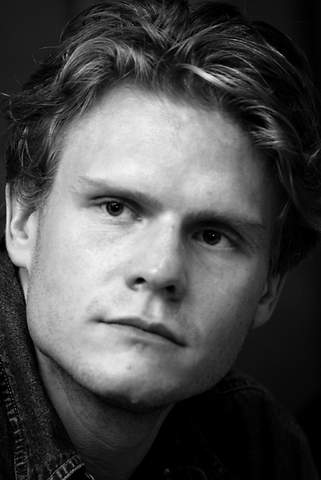
\includegraphics[scale=0.3]{./imgs/profilepic2.jpg}
\end{center}
\end{column}
\begin{column}{0.6\columnwidth}
Willy Rempel
\begin{itemize}
\item HBSc Computer Science \\
\item BSc Mathematics \\
\item Research Associate, AISC \\
\item seeking opportunities in the field
\end{itemize}
\end{column}
\end{columns}
\end{frame}
\begin{frame}[label={sec:org54c1d38}]{Introduction}
\begin{quote}
Although all of the ideas in the model are doubtlessly clever, the main secret behind AlphaFold 2’s success is the superb deep learning engineering. A close look at the model reveals an architecture with a large amount of small details that seem fundamental for the performance of the network. As we admire the end product, we should not turn a blind eye to the enormous budget, and the large team of full-time, handsomely paid engineers that made it possible.  \cite{rubieraAlphaFoldHereWhat}
\end{quote}

\begin{quote}
This, and many other tricks, are described in exhaustive detail in the Supplementary Information. A reduced subset has been analysed in a brief ablation study, but ultimately, how important are each of the minor details is anybody’s guess.  \cite{rubieraAlphaFoldHereWhat}
\end{quote}

\flushright{(above blog post is recommended reading)}
\end{frame}
\begin{frame}[label={sec:orgd0a1090}]{Model Overview \cite{jumperHighlyAccurateProtein2021}}
\begin{center}
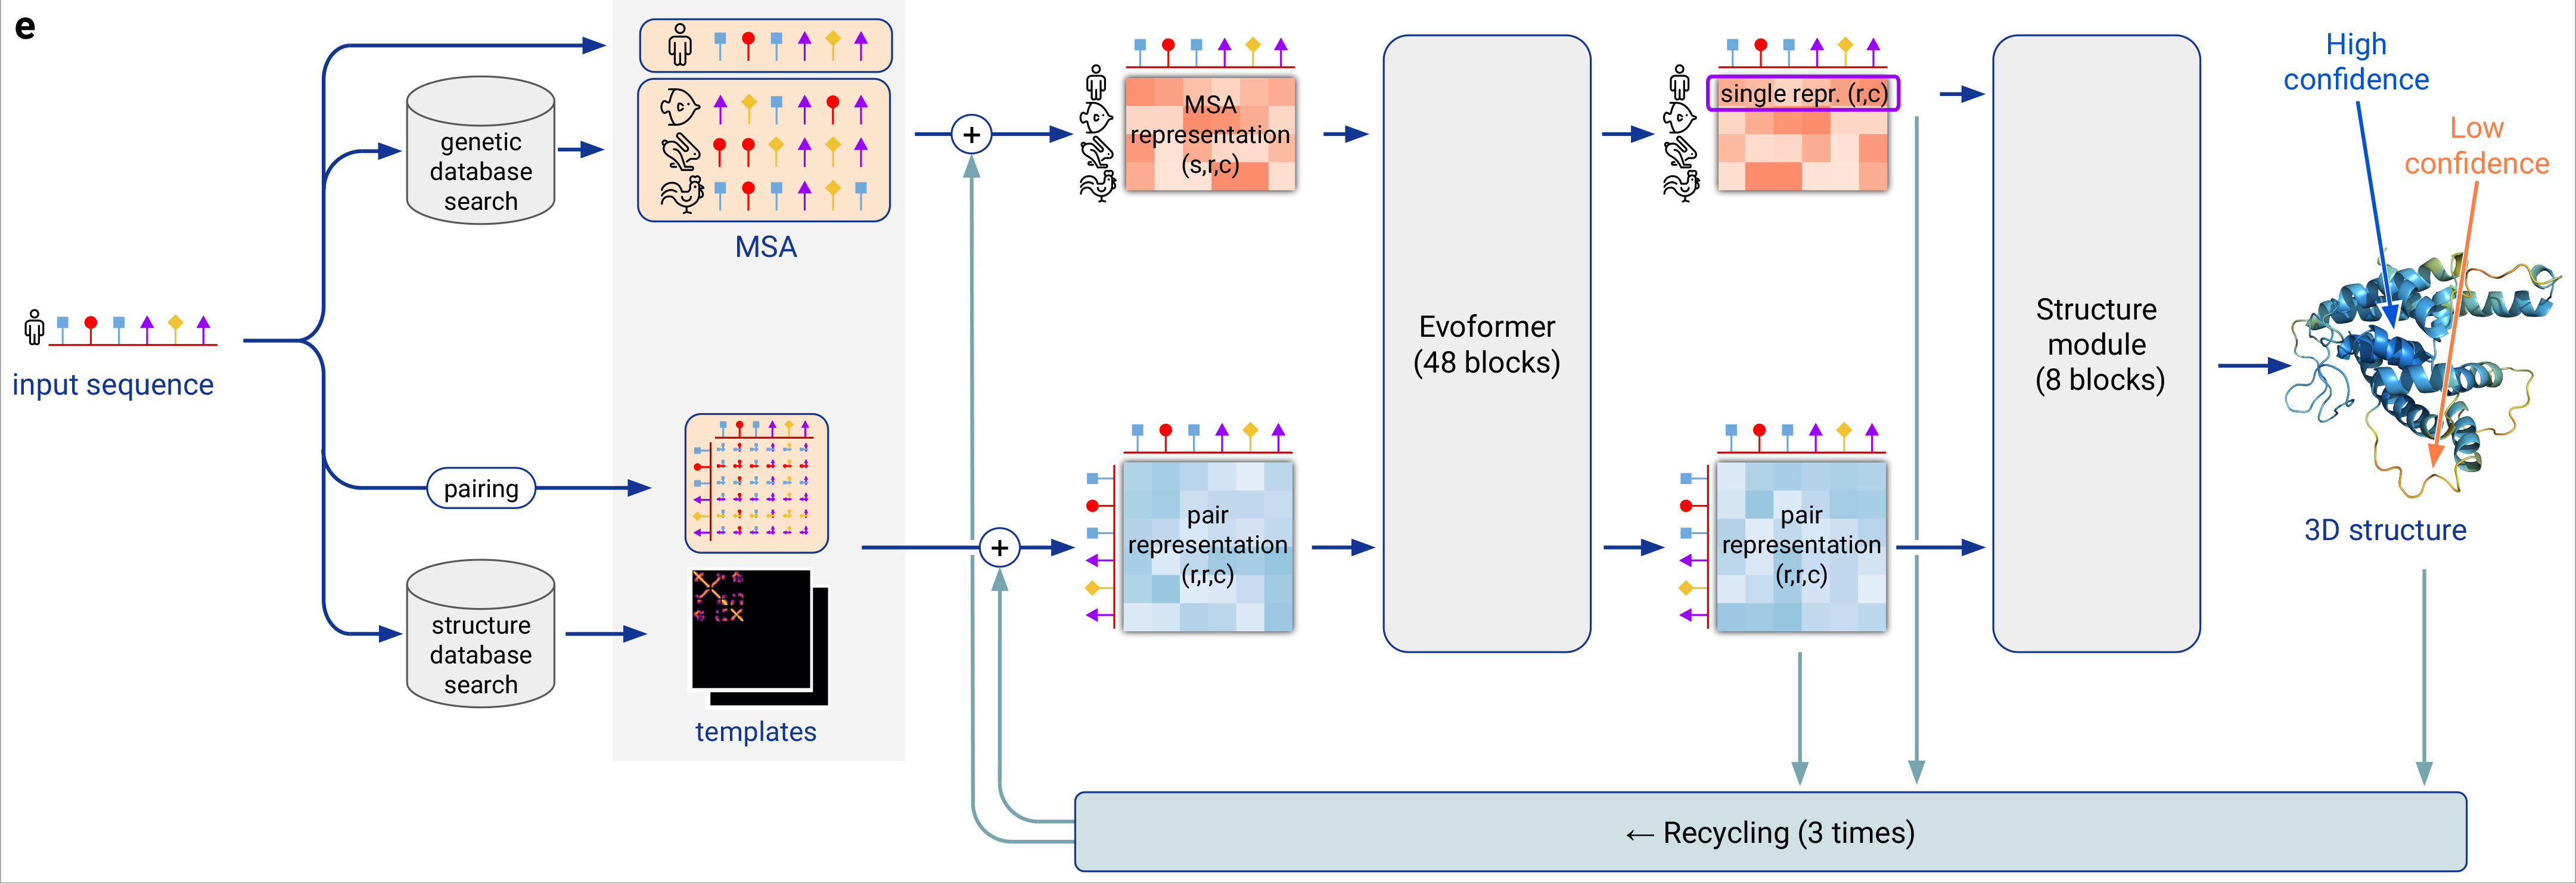
\includegraphics[width=.9\linewidth]{./imgs/model-overview.png}
\end{center} 
\end{frame}

\section*{Data Pipeline}
\label{sec:org11d2f66}
\begin{frame}[label={sec:orgc2d4375}]{Initial Input: mmCIF or FASTA files}
\begin{center}
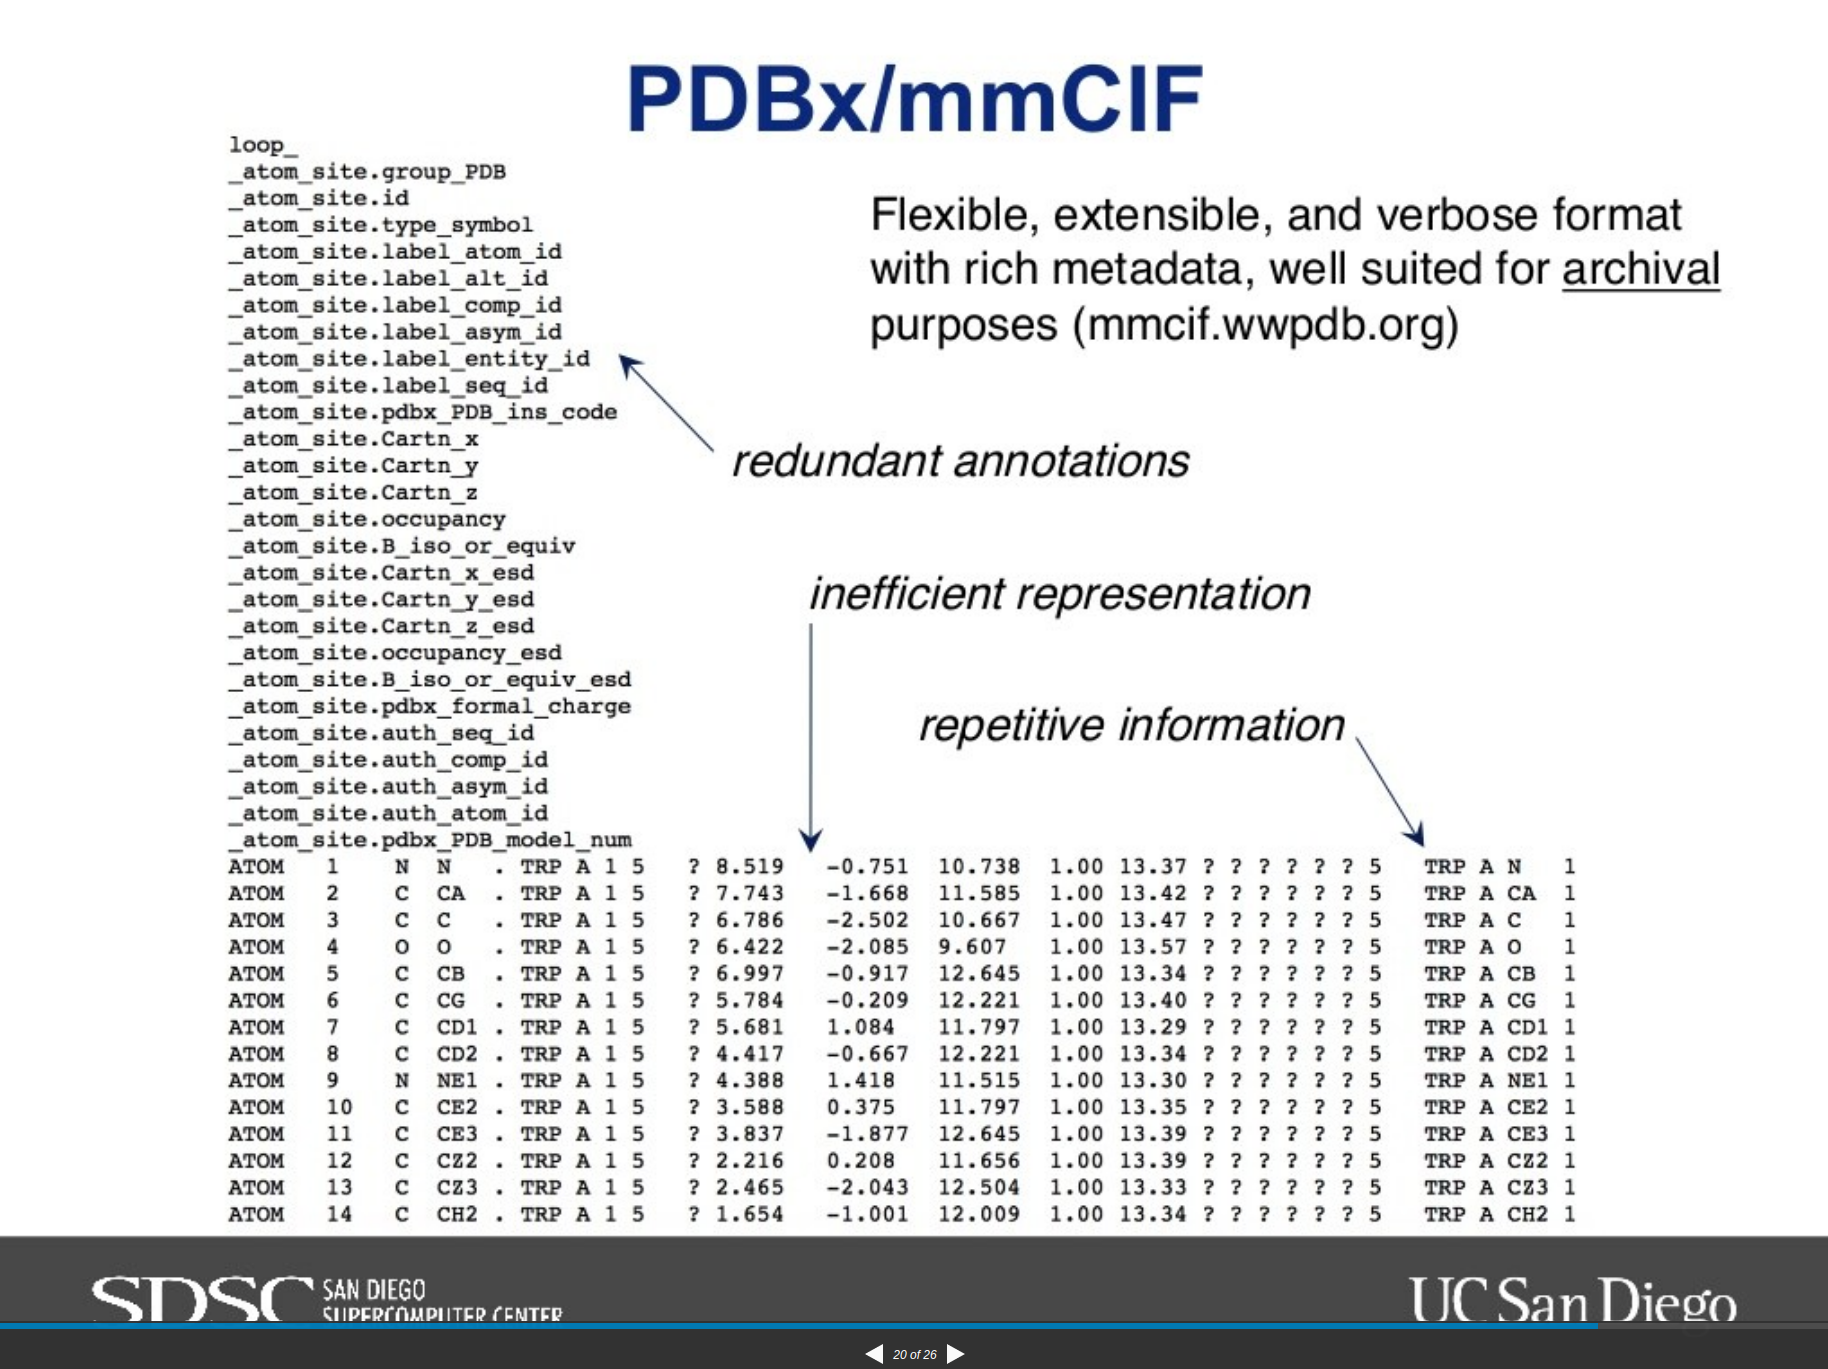
\includegraphics[width=.9\linewidth]{./imgs/mmcif-eg.png}
\end{center}

see \cite{PDB101LearnGuide} for full guide
\end{frame}

\begin{frame}[label={sec:orga763d79}]{Initial Input: mmCIF or FASTA files}
\begin{center}
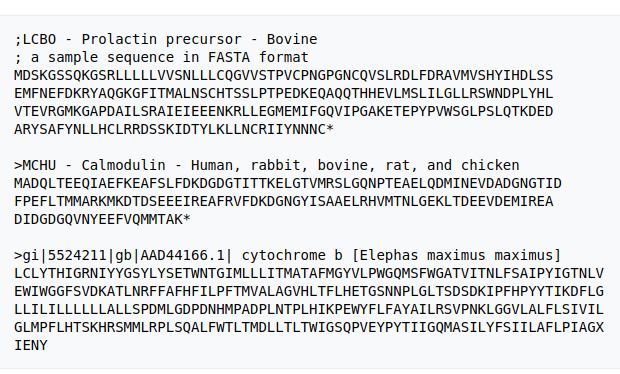
\includegraphics[width=.9\linewidth]{./imgs/fastafiles_2021-07-20.png}
\end{center}
\end{frame}

\begin{frame}[label={sec:org192b794}]{Parsing \cite{jumperHighlyAccurateProtein2021}}
\begin{itemize}
\item only certain metadata (more from mmCIF)
\item change MSE residues into MET
\end{itemize}
\end{frame}

\begin{frame}[label={sec:org4ee7e1b}]{Genetic Search \cite{jumperHighlyAccurateProtein2021}}
For MSAs
\begin{itemize}
\item JackHMMER
\begin{itemize}
\item MGnify: MSA depth 5,000
\item UniRef90: MSA depth 10,000
\end{itemize}
\item HHBlits
\begin{itemize}
\item Uniclust30 + BFD: MSA depth unlimited
\end{itemize}
\item MSAs duplicated and stacked
\end{itemize}

flags:
  JackHMMER: -N 1 -E 0.0001 --incE 0.0001 --F1 0.0005 --F2 0.00005 --F3 0.0000005.
  HHBlits: -n 3 -e 0.001 -realign\textsubscript{max} 100000 -maxfilt 100000 -min\textsubscript{prefilter}\textsubscript{hits} 1000 -maxseq 1000000.
\end{frame}

\begin{frame}[label={sec:orgba511fa}]{Template Search \cite{jumperHighlyAccurateProtein2021}}
\begin{itemize}
\item UniRef90 MSA from prior search used for PDB70 search using HHSearch.
\item Filter out:
\begin{itemize}
\item released after the input sequence
\item or identical to the input sequence
\item too small
\end{itemize}
\item At inference use top 4 templates
\end{itemize}
\end{frame}

\begin{frame}[label={sec:orgd22cd9e}]{Training Data \cite{jumperHighlyAccurateProtein2021}}
\begin{itemize}
\item 75:25 self-distillation : known structure (PDB)
\item stochastic filters (next)
\end{itemize}
\end{frame}

\begin{frame}[label={sec:org75da01b}]{Filtering \cite{jumperHighlyAccurateProtein2021}}
\begin{itemize}
\item stochastic filters: 
\begin{itemize}
\item Input mmCIFs are restricted to have resolution less than 9 Å. This is not a very restrictive filter and only removes around 0.2\% of structures.
\item Longer protein chains are selected with higher probability.
\item Also favour protein chains from smaller clusters. They use 40\% sequence identity clusters of the Protein Data Bank clustered with MMSeqs2.
\item Sequences are filtered out when any single amino acid accounts for more than 80\% of the input primary sequence. This filter removes about 0.8\% of sequences.
\end{itemize}
\end{itemize}
\end{frame}

\begin{frame}[label={sec:org04257b4}]{MSA block deletion \cite{jumperHighlyAccurateProtein2021}}
\begin{itemize}
\item MSAs grouped by tool, sorted by block output? (e-value?)
\begin{itemize}
\item similar sequences are likely to be adjacent
\item block deletion tends to remove similarities (ie. whole branch phylogeny)
\end{itemize}
\end{itemize}
\end{frame}

\begin{frame}[label={sec:orgdf8c8ab}]{MSA clustering \cite{jumperHighlyAccurateProtein2021}}
\begin{itemize}
\item Similarity clusters used to randomly select subset of MSA sequences 
\begin{itemize}
\item to reduce computational cost from attention modules, reduce \(N_seq\)
\end{itemize}

\item K-means, input sequence used as first cluster center
\item masking
\item hamming distance measure for remaining selections
\end{itemize}
\end{frame}

\begin{frame}[label={sec:org2fbaab8}]{Residue cropping \cite{jumperHighlyAccurateProtein2021}}
During training:
\begin{enumerate}
\item unclamped \& clamped - sampling start index from uniform distributions
\item Cropped with fixed size \(N_res\)
\end{enumerate}
\end{frame}

\begin{frame}[label={sec:org6a2235d}]{Featurization and model inputs \cite{jumperHighlyAccurateProtein2021}}
\begin{itemize}
\item \alert{target\textsubscript{feat}}
This is a feature of size [Nres, 21] consisting of the “aatype” feature.
\item \alert{residue\textsubscript{index}}
This is a feature of size [Nres] consisting of the “residue\textsubscript{index}” feature.
\item \alert{msa\textsubscript{feat}}
This is a feature of size [Nclust, Nres, 49] constructed by concatenating “cluster\textsubscript{msa}”, “cluster\textsubscript{has}\textsubscript{deletion}”, “cluster\textsubscript{deletion}\textsubscript{value}”, “cluster\textsubscript{deletion}\textsubscript{mean}”, “cluster\textsubscript{profile}”. We draw Ncycle×Nensemble random samples from this feature to provide each recycling/ensembling iteration of the network with a different sample (see subsubsection 1.11.2).
\item \alert{extra\textsubscript{msa}\textsubscript{feat}}
This is a feature of size [Nextra\textsubscript{seq}, Nres, 25] constructed by concatenating “extra\textsubscript{msa}”, “extra\textsubscript{msa}\textsubscript{has}\textsubscript{deletion}”, “extra\textsubscript{msa}\textsubscript{deletion}\textsubscript{value}”. Together with “msa\textsubscript{feat}’ above we also draw Ncycle × Nensemble random samples from this feature (see subsubsection 1.11.2).
\end{itemize}
\end{frame}
\begin{frame}[label={sec:org7e6b480}]{Featurization and model inputs \cite{jumperHighlyAccurateProtein2021}}
\begin{itemize}
\item \alert{template\textsubscript{pair}\textsubscript{feat}}
This is a feature of size [Ntempl, Nres, Nres, 88] and consists of concatenation of the pair residue features “template\textsubscript{distogram}”, “template\textsubscript{unit}\textsubscript{vector}”, and also several residue features, which are transformed into pair features. The “template\textsubscript{aatype}” feature is included via tiling and stack- ing (this is done twice, in both residue directions). Also the mask features “template\textsubscript{pseudo}\textsubscript{beta}\textsubscript{mask}” and “template\textsubscript{backbone}\textsubscript{frame}\textsubscript{mask}” are included, where the feature fij = maski · maskj. - template\textsubscript{angle}\textsubscript{feat} This is a feature of size [Ntempl, Nres, 51] constructed by concatenating the following features: “template\textsubscript{aatype}”, “template\textsubscript{torsion}\textsubscript{angles}”, “template\textsubscript{alt}\textsubscript{torsion}\textsubscript{angles}”, and “template\textsubscript{torsion}\textsubscript{angles}\textsubscript{mask}”.
\end{itemize}
\end{frame}

\begin{frame}[label={sec:org372eecf}]{Self-distillation dataset \cite{jumperHighlyAccurateProtein2021}}
\begin{itemize}
\item Build dataset (on unlabeled sequences):
\begin{enumerate}
\item Make MSA for every cluster in Uniclust30
\item Remove sequences that appear in another sequences MSA
\item Keep sequences of 200 < length < 1024
\item Remove sequences where MSA < 200 alignments
\end{enumerate}
\item For predicted structures:
\begin{itemize}
\item train 'undistlled' model on just PDB dataset
\item use this model to predict above set
\item for every residue pair, computer confidence metric using KL-divergence between distance distribution and a reference distribution
\item reference distribution
\end{itemize}
\item self-distillation training took \textasciitilde{}2 weeks
\end{itemize}
\end{frame}

\section*{Model Architecture}
\label{sec:org75d8915}
\begin{frame}[label={sec:orgc31605c}]{Input embeddings \cite{jumperHighlyAccurateProtein2021}}
\begin{center}
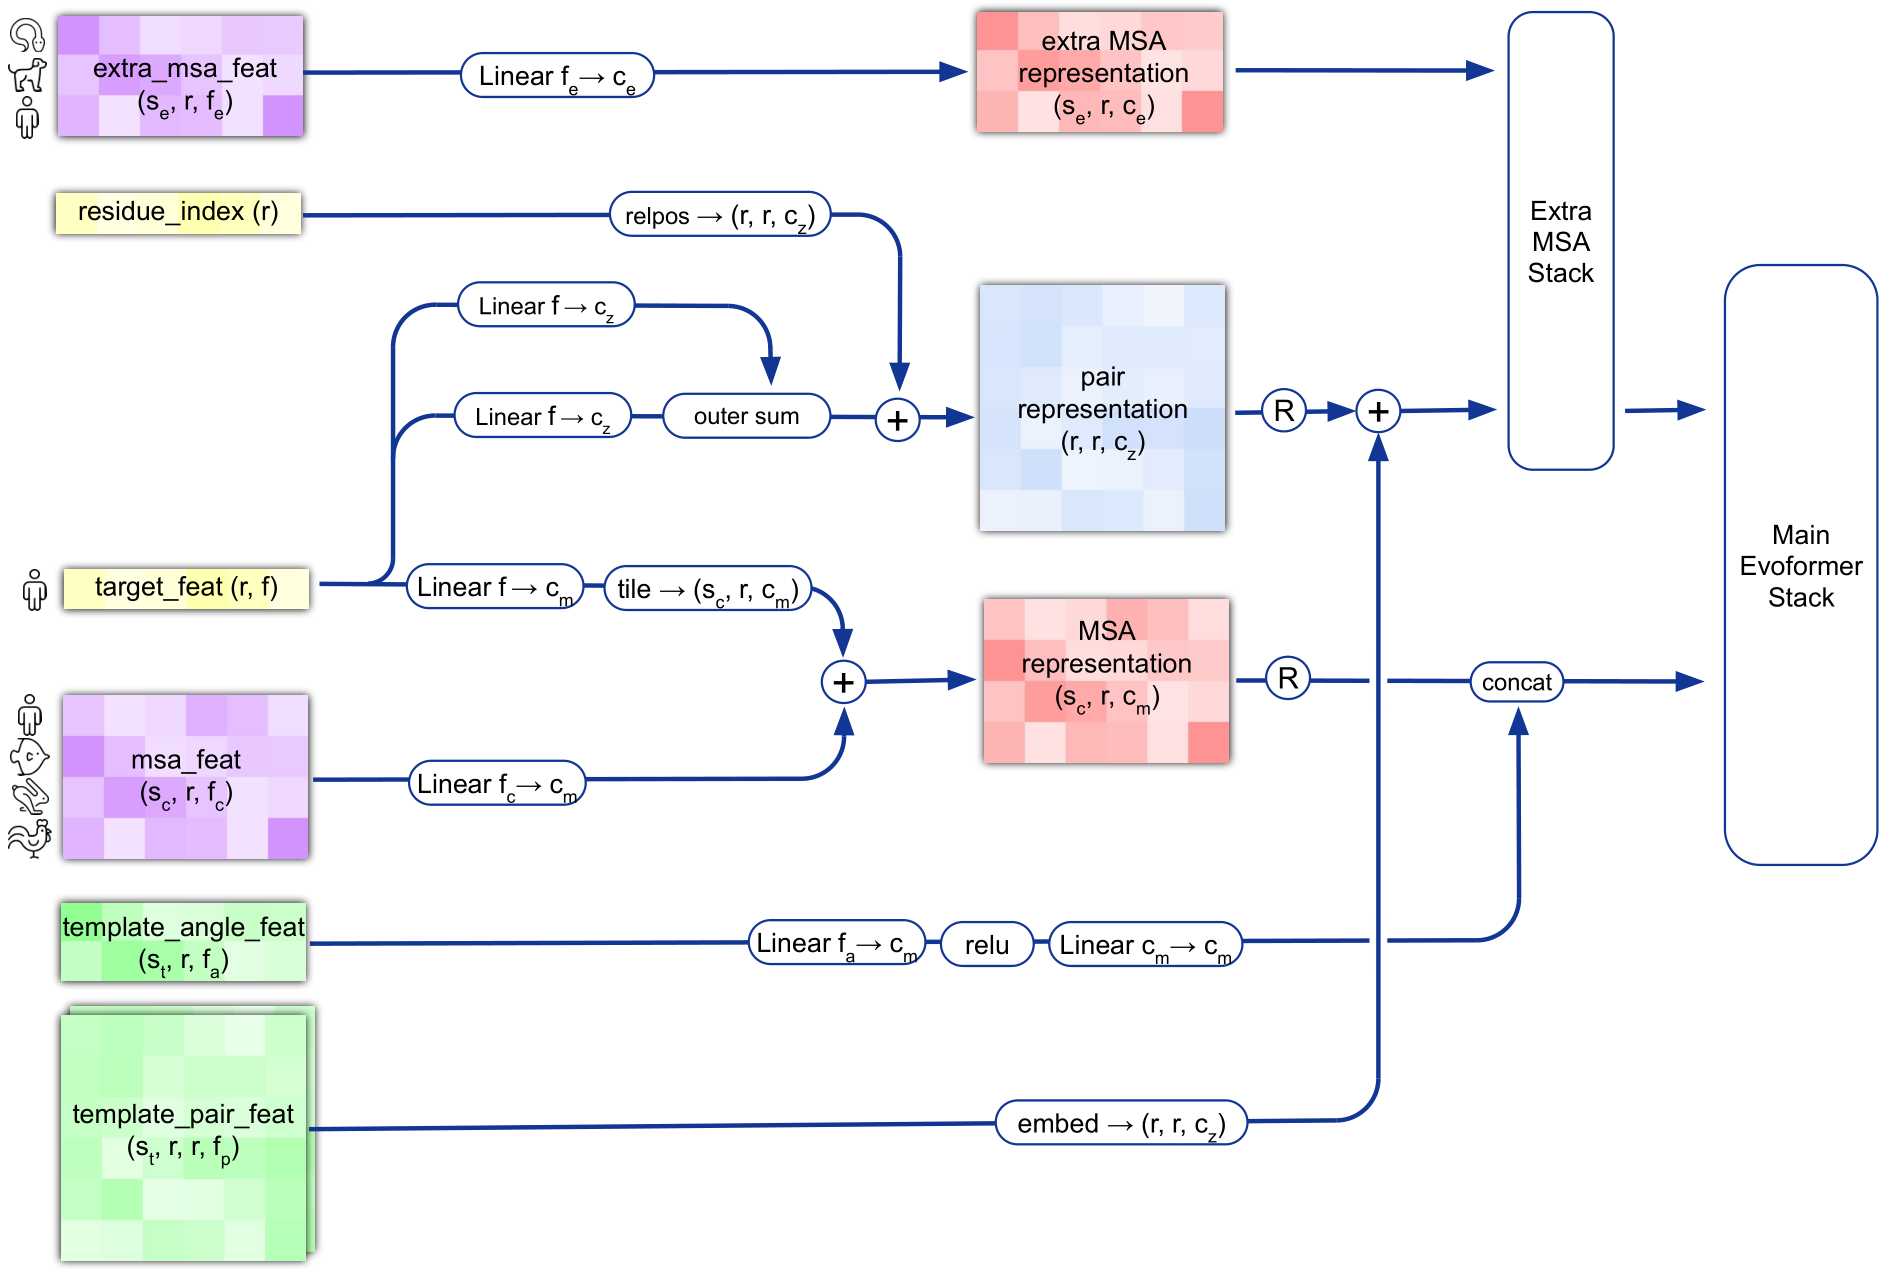
\includegraphics[height=\textheight]{./imgs/input_embeddings.png}
\end{center}
\cite{jumperHighlyAccurateProtein2021}
\end{frame}
\subsection*{EvoFormer}
\label{sec:orga028468}
\begin{frame}[label={sec:orge6ac59d}]{EvoFormer: Overview \cite{jumperHighlyAccurateProtein2021}}
\begin{center}
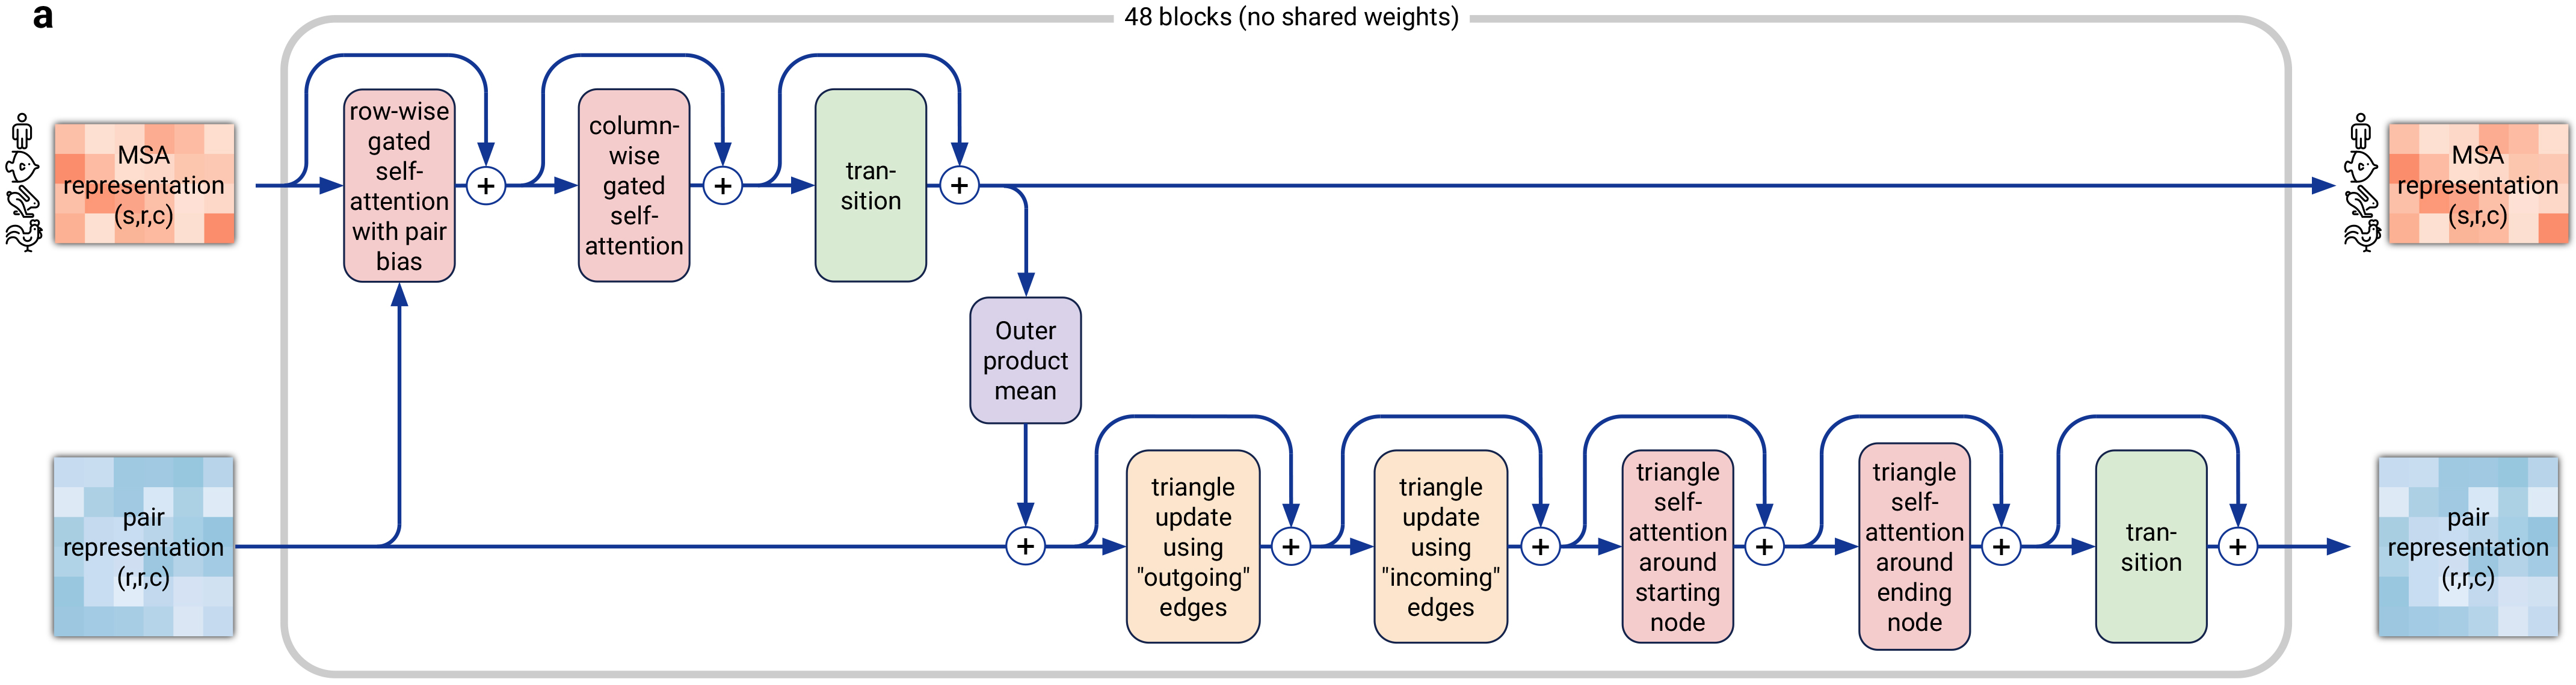
\includegraphics[width=.9\linewidth]{./imgs/model-evoformer-main.png}
\end{center} 
\end{frame}

\begin{frame}[label={sec:org8063773}]{EvoFormer: Overview \cite{jumperHighlyAccurateProtein2021}}
\begin{itemize}
\item cast as a graph inference problem
\item cross-optimization and information flow between MSA representation and pair-wise representation
\item layer normalization
\end{itemize}
\end{frame}

\begin{frame}[label={sec:orgb477dba}]{EvoFormer: Row wise Gated Attention \cite{jumperHighlyAccurateProtein2021}}
\begin{center}
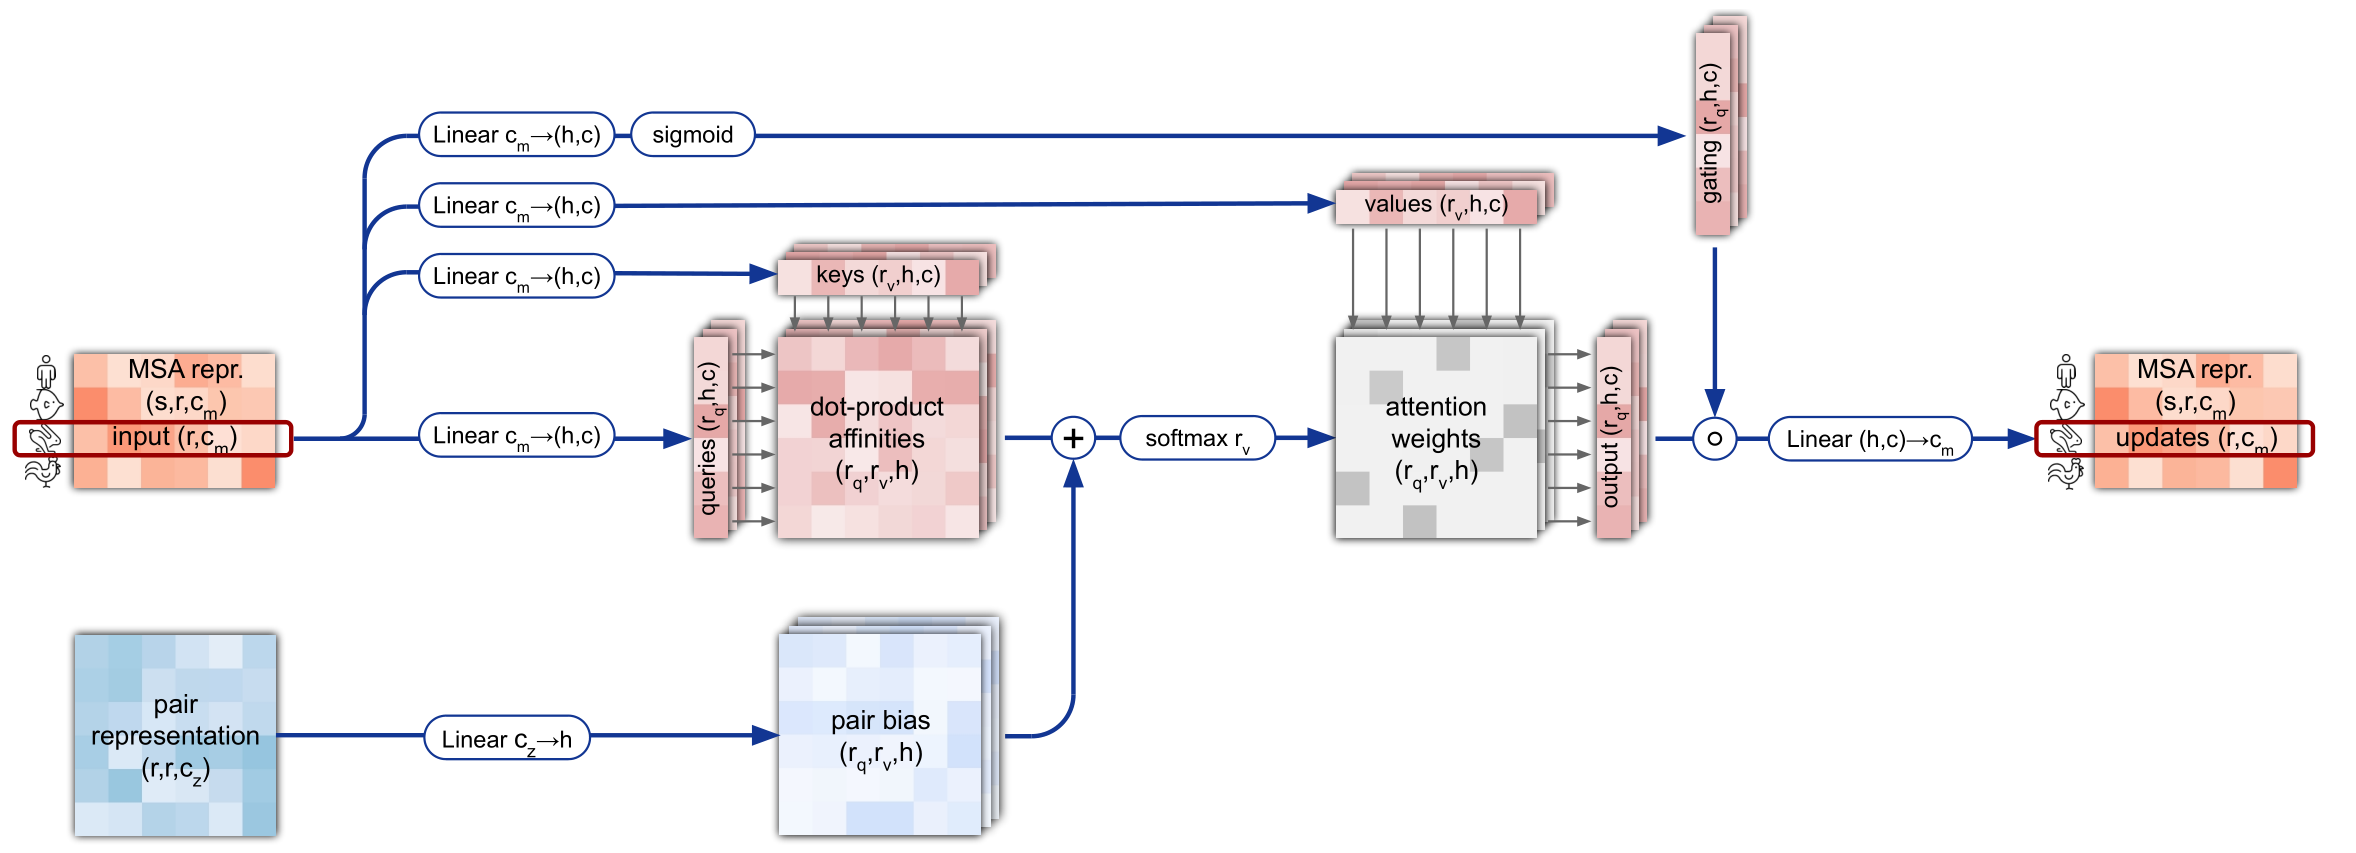
\includegraphics[width=.9\linewidth]{./imgs/rowwise-gated-attention.png}
\end{center}
\end{frame}

\begin{frame}[label={sec:org1602926}]{EvoFormer: Column wise Gated Attention \cite{jumperHighlyAccurateProtein2021}}
\begin{center}
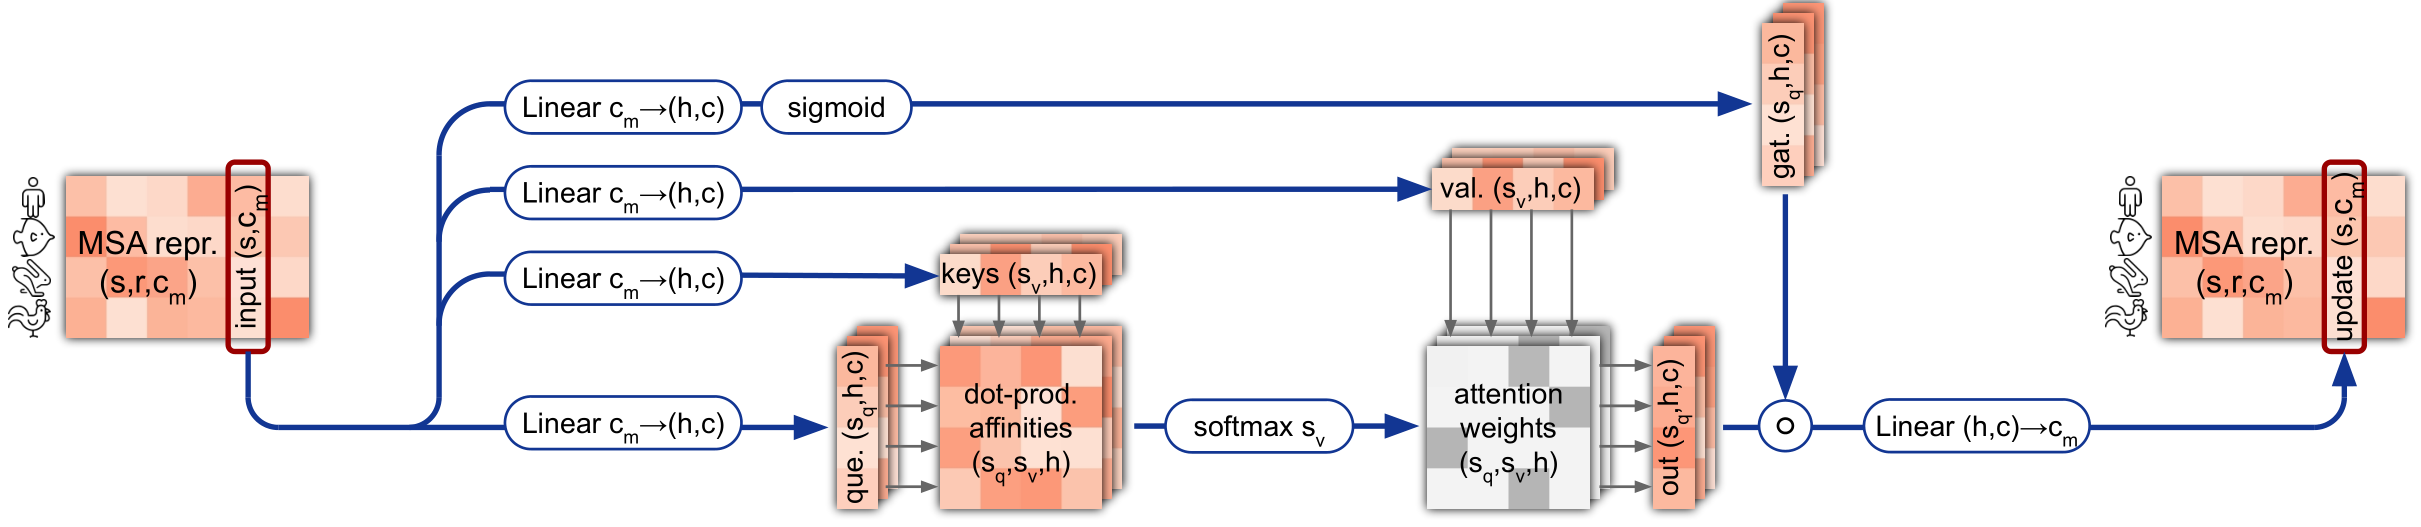
\includegraphics[width=.9\linewidth]{./imgs/columnwise-gated-attention.png}
\end{center}
\end{frame}

\begin{frame}[label={sec:org93dc13e}]{EvoFormer: MSA Translation Layer \cite{jumperHighlyAccurateProtein2021}}
\begin{center}
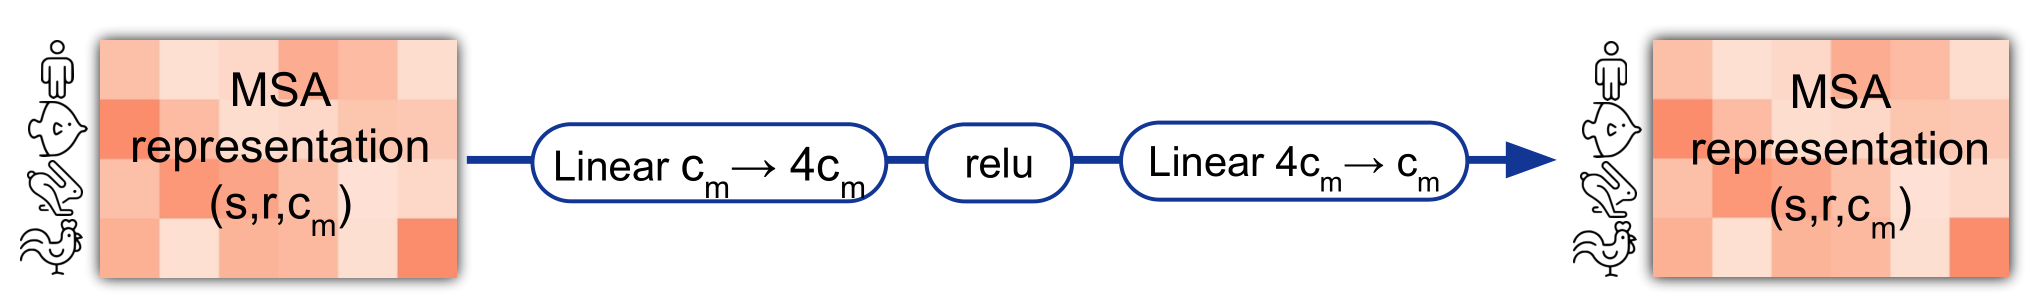
\includegraphics[width=.9\linewidth]{./imgs/msa-translation-layer.png}
\end{center}
\end{frame}

\begin{frame}[label={sec:org2d98481}]{EvoFormer: Outer-Product Mean \cite{jumperHighlyAccurateProtein2021}}
\begin{center}
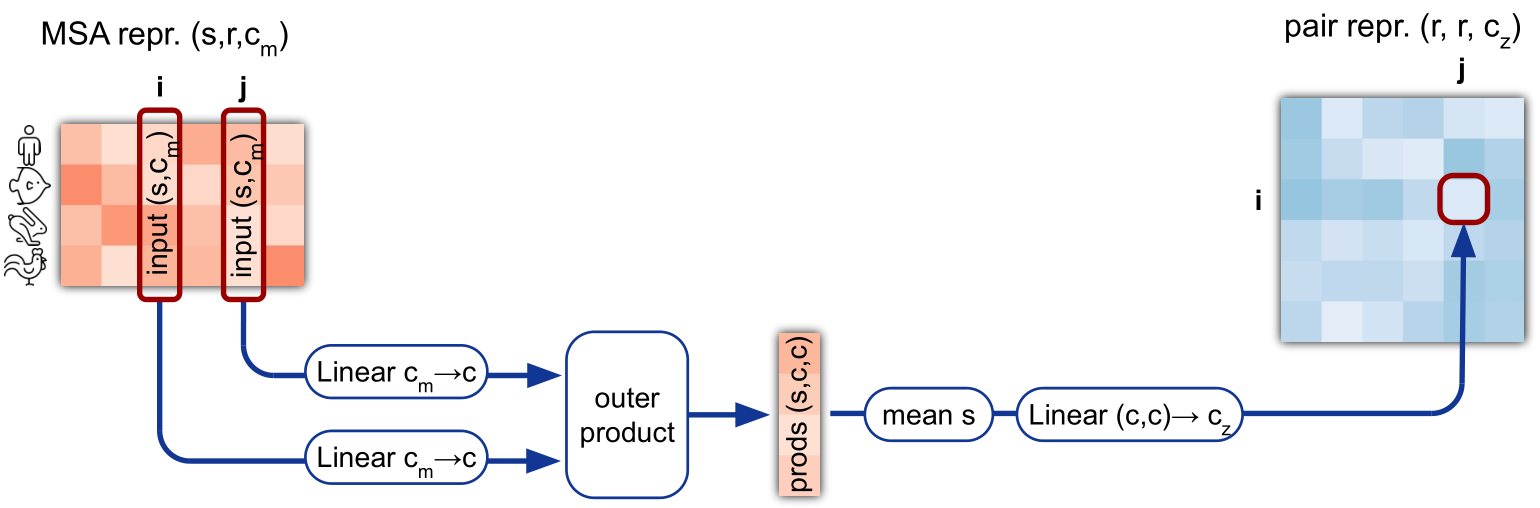
\includegraphics[width=.9\linewidth]{./imgs/outer-product-mean.png}
\end{center}
\end{frame}

\begin{frame}[label={sec:org59b1a86}]{EvoFormer: Residue Pairs \cite{jumperHighlyAccurateProtein2021}}
\begin{center}
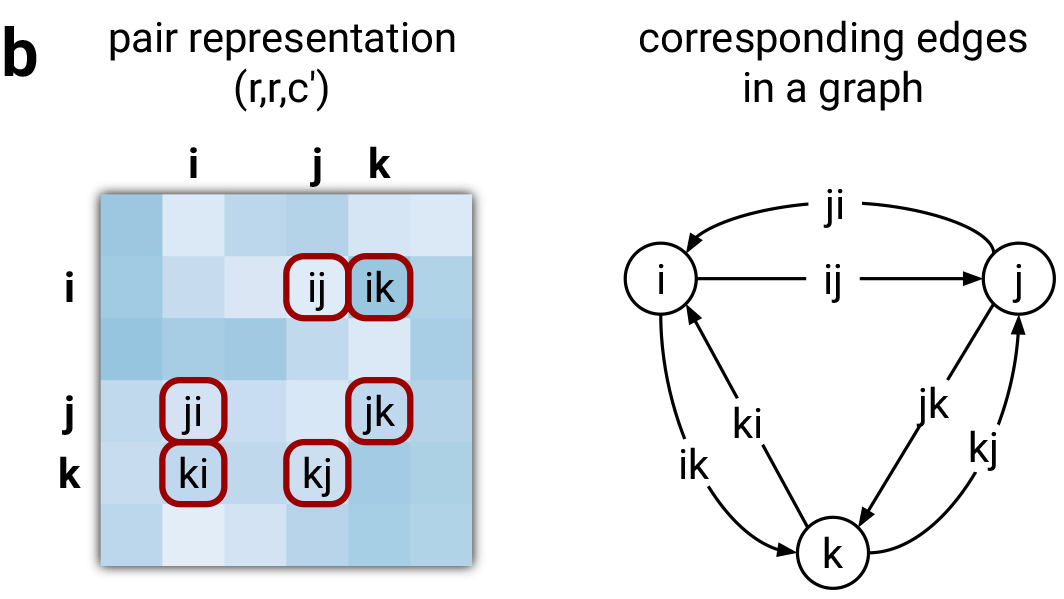
\includegraphics[scale=0.25]{./imgs/model-evoformer-pair1.png}
\end{center}
\begin{center}
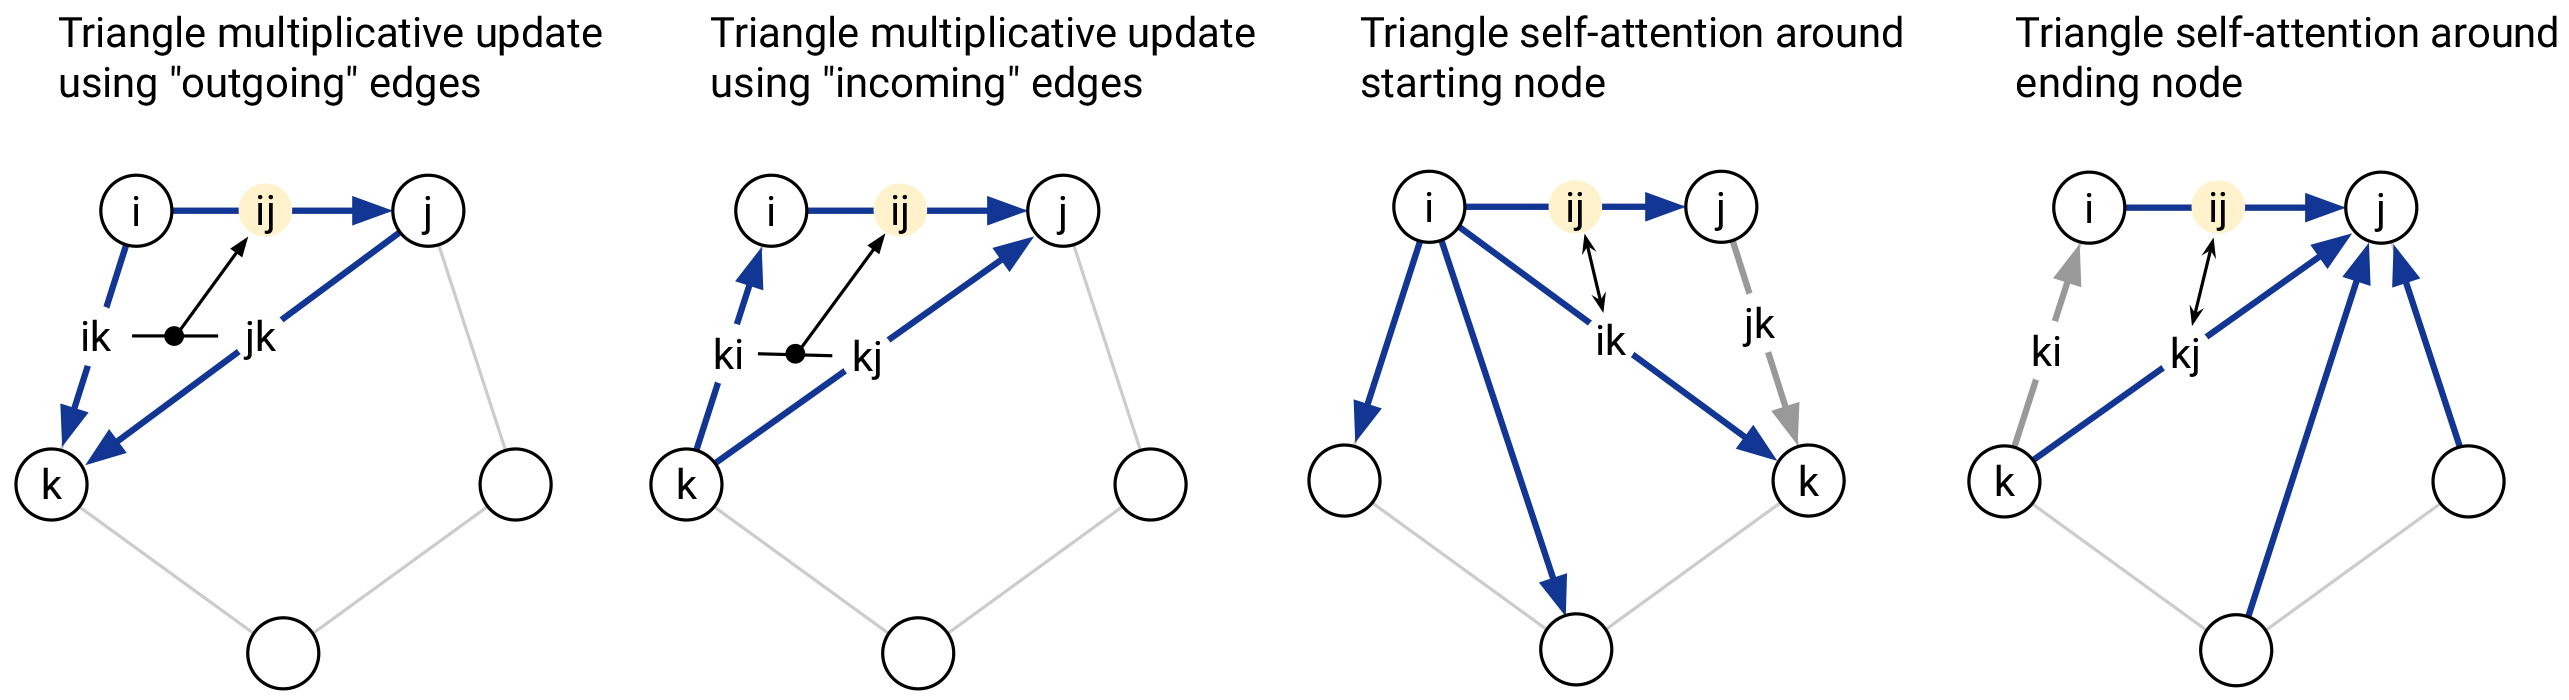
\includegraphics[width=.9\linewidth]{./imgs/model-evoformer-pair2.png}
\end{center}
\end{frame}

\begin{frame}[label={sec:orgf150cd4}]{EvoFormer: Triangular Multiplicative Update \cite{jumperHighlyAccurateProtein2021}}
\begin{center}
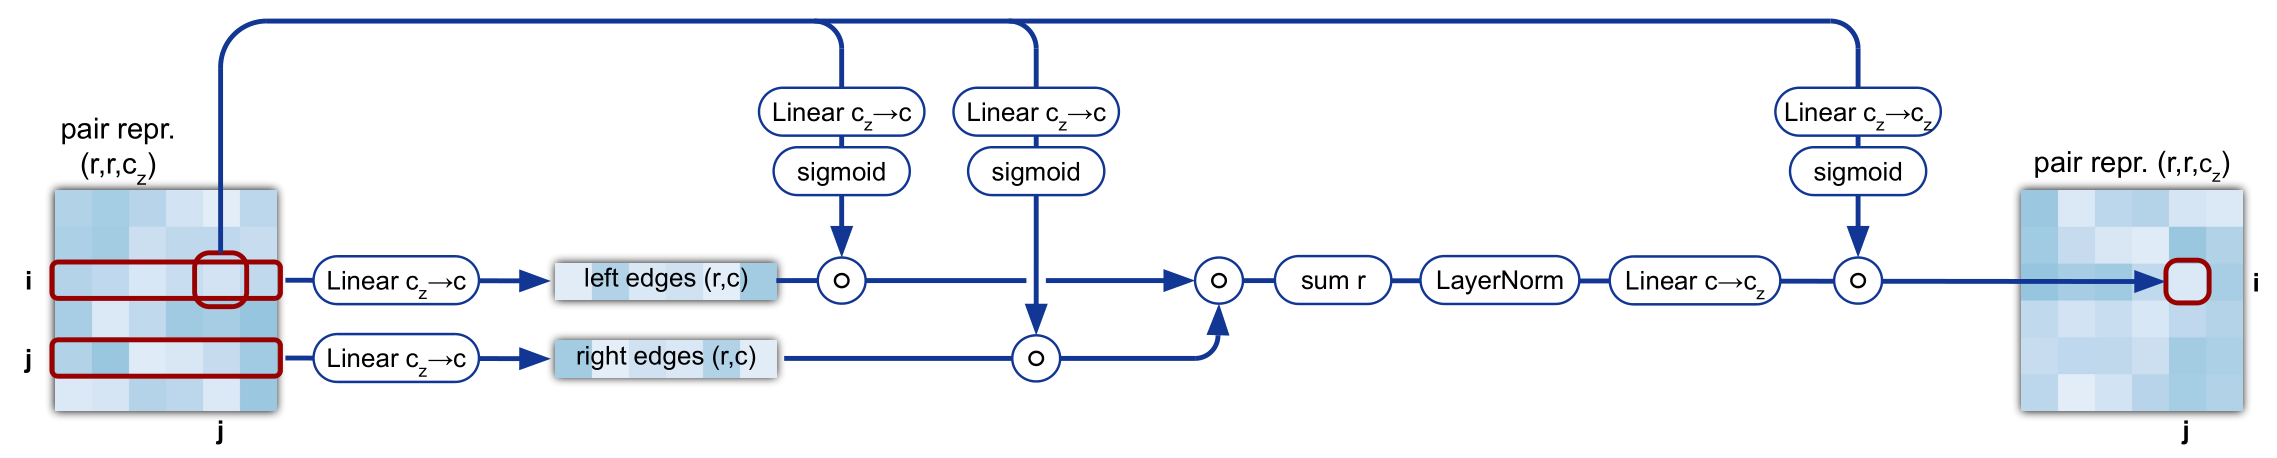
\includegraphics[width=.9\linewidth]{./imgs/triangular-mult-update.png}
\end{center}
\end{frame}

\begin{frame}[label={sec:org8ee6e22}]{EvoFormer: Triangular Self-Attention \cite{jumperHighlyAccurateProtein2021}}
\begin{center}
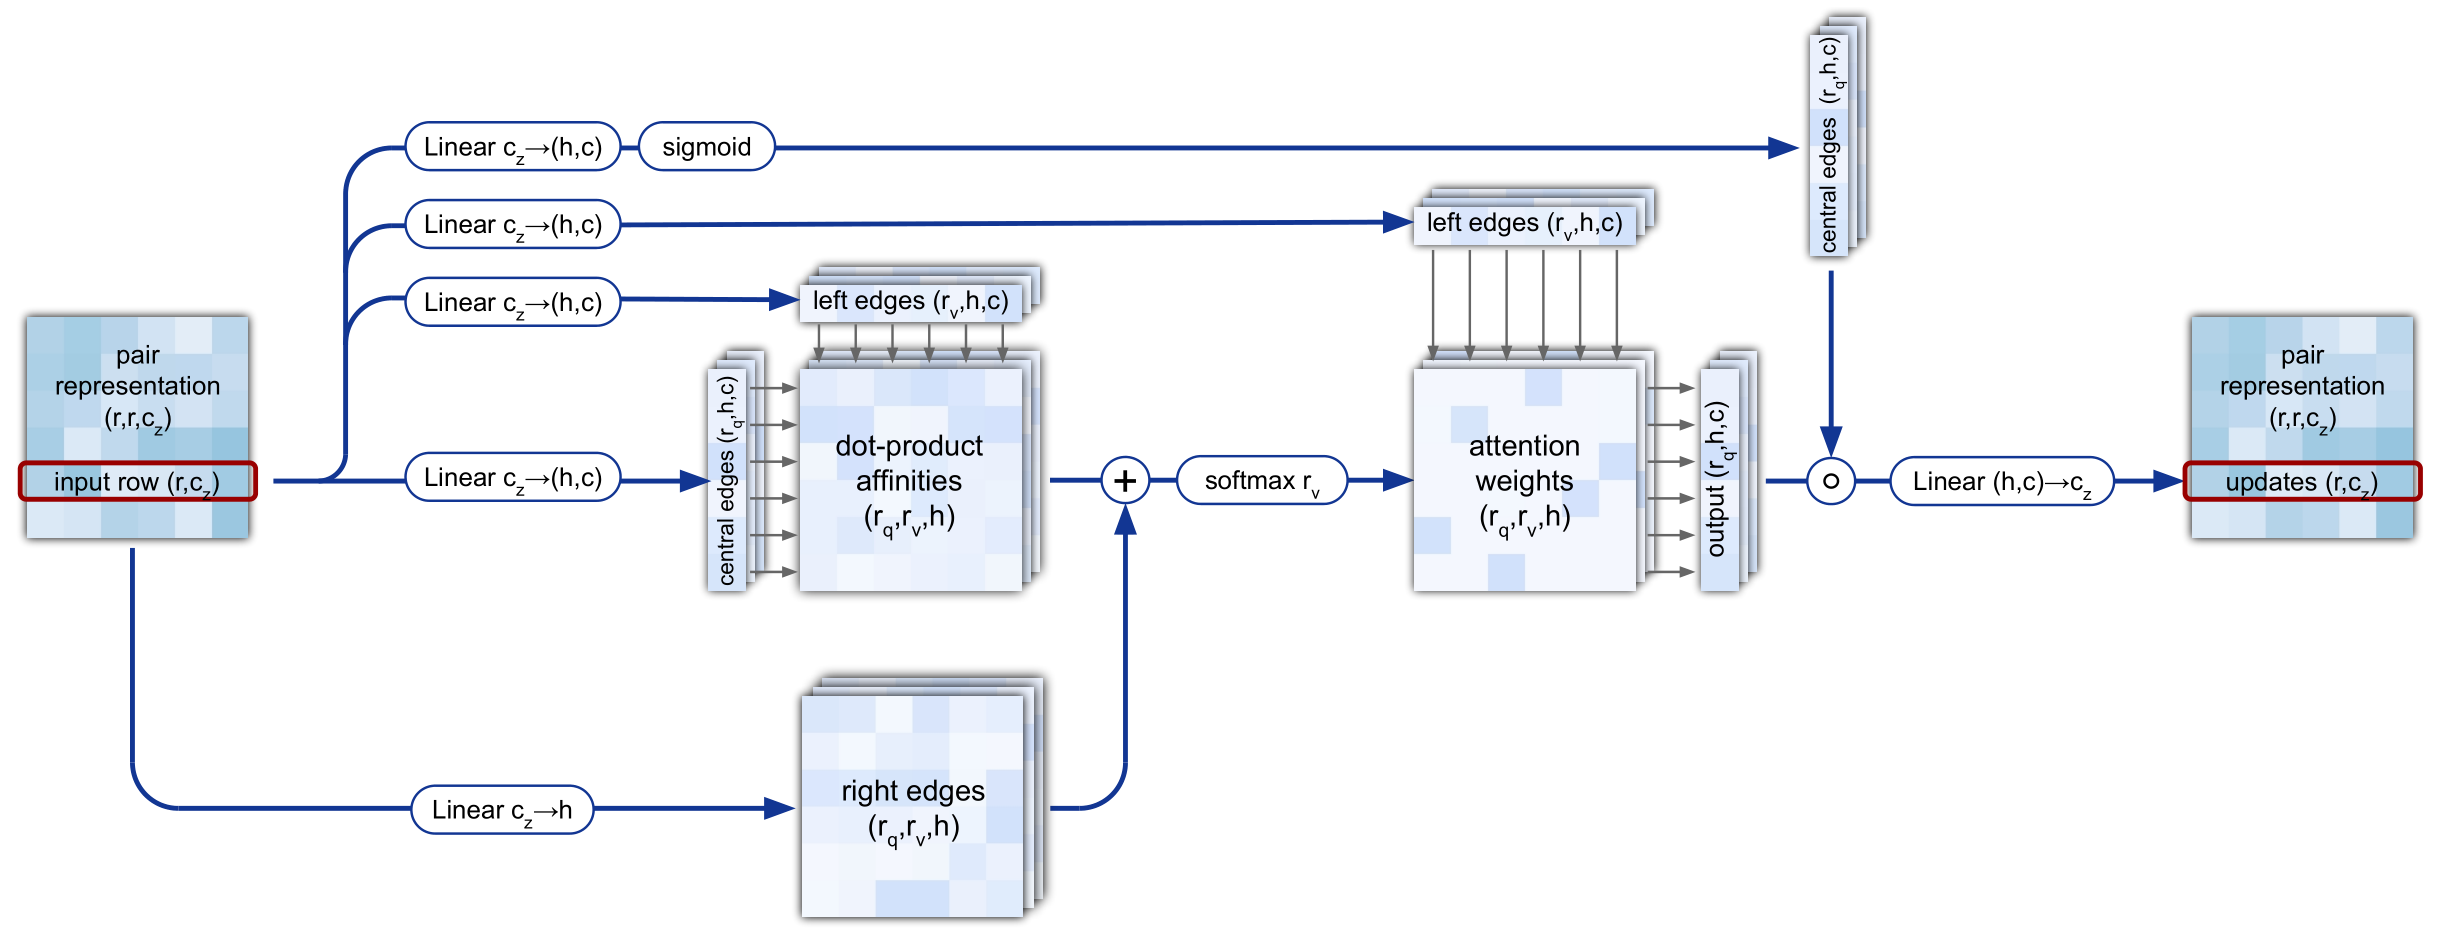
\includegraphics[width=.9\linewidth]{./imgs/triangular-self-attention.png}
\end{center}
\end{frame}

\subsection*{Structure Module}
\label{sec:orgb2dec5f}
\begin{frame}[label={sec:org758e7f0}]{Structure Module: Overview \cite{jumperHighlyAccurateProtein2021}}
\begin{center}
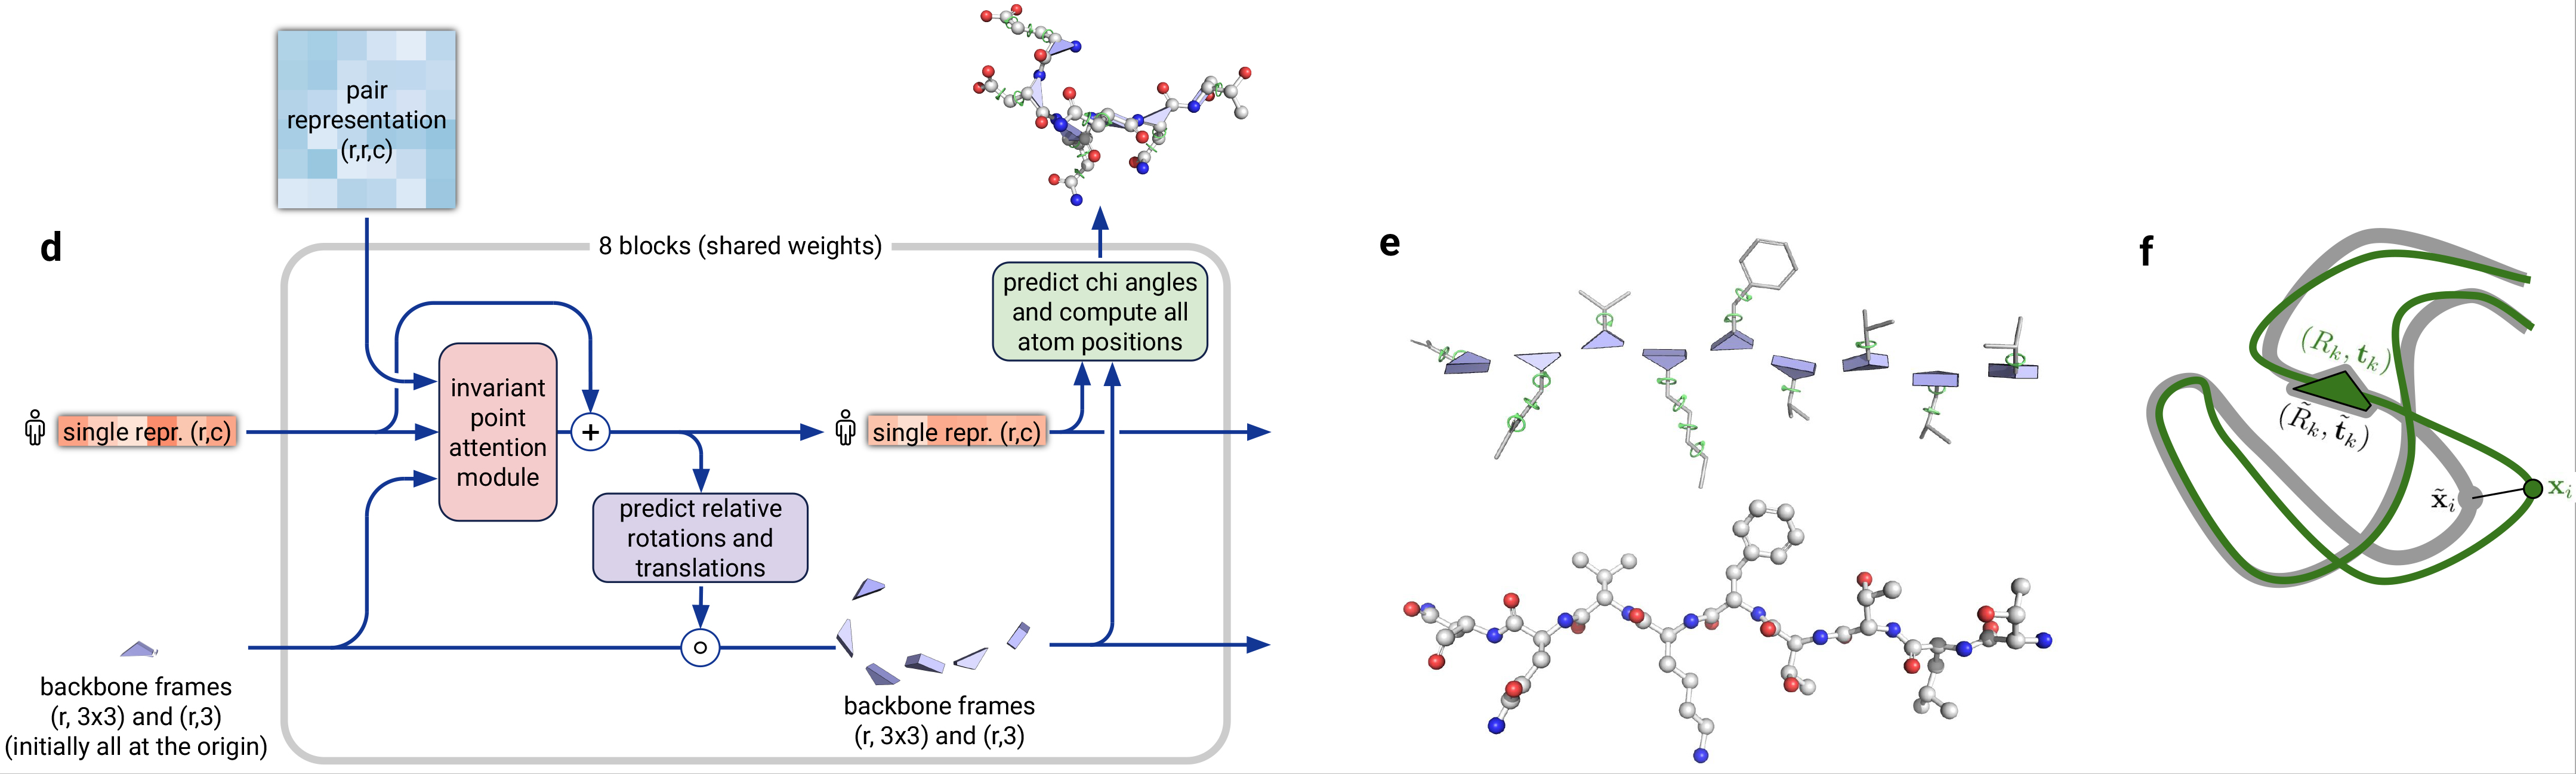
\includegraphics[width=.9\linewidth]{./imgs/model-structure.png}
\end{center}
\end{frame}

\begin{frame}[label={sec:orgcd6ca1b}]{Structure Module: Frame Representation}
\begin{figure}[htbp]
\centering
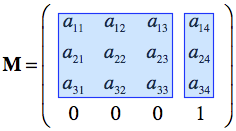
\includegraphics[width=.9\linewidth]{./imgs/TransformationMatrix1.png}
{Example transform cite:SpatialTransformationMatrices}
\end{figure}

\begin{itemize}
\item rotation + translation transforms \(T_i := (R_i,t_i)\)
\item no reflection, scaling, or shear
\item they construct ground truth frames using the position of three atoms from the ground truth PDB structures using a Gram–Schmidt process (Algorithm 21)
\end{itemize}
\end{frame}
\begin{frame}[label={sec:orgfcdc878}]{Structure Module: IPA \cite{jumperHighlyAccurateProtein2021}}
\begin{center}
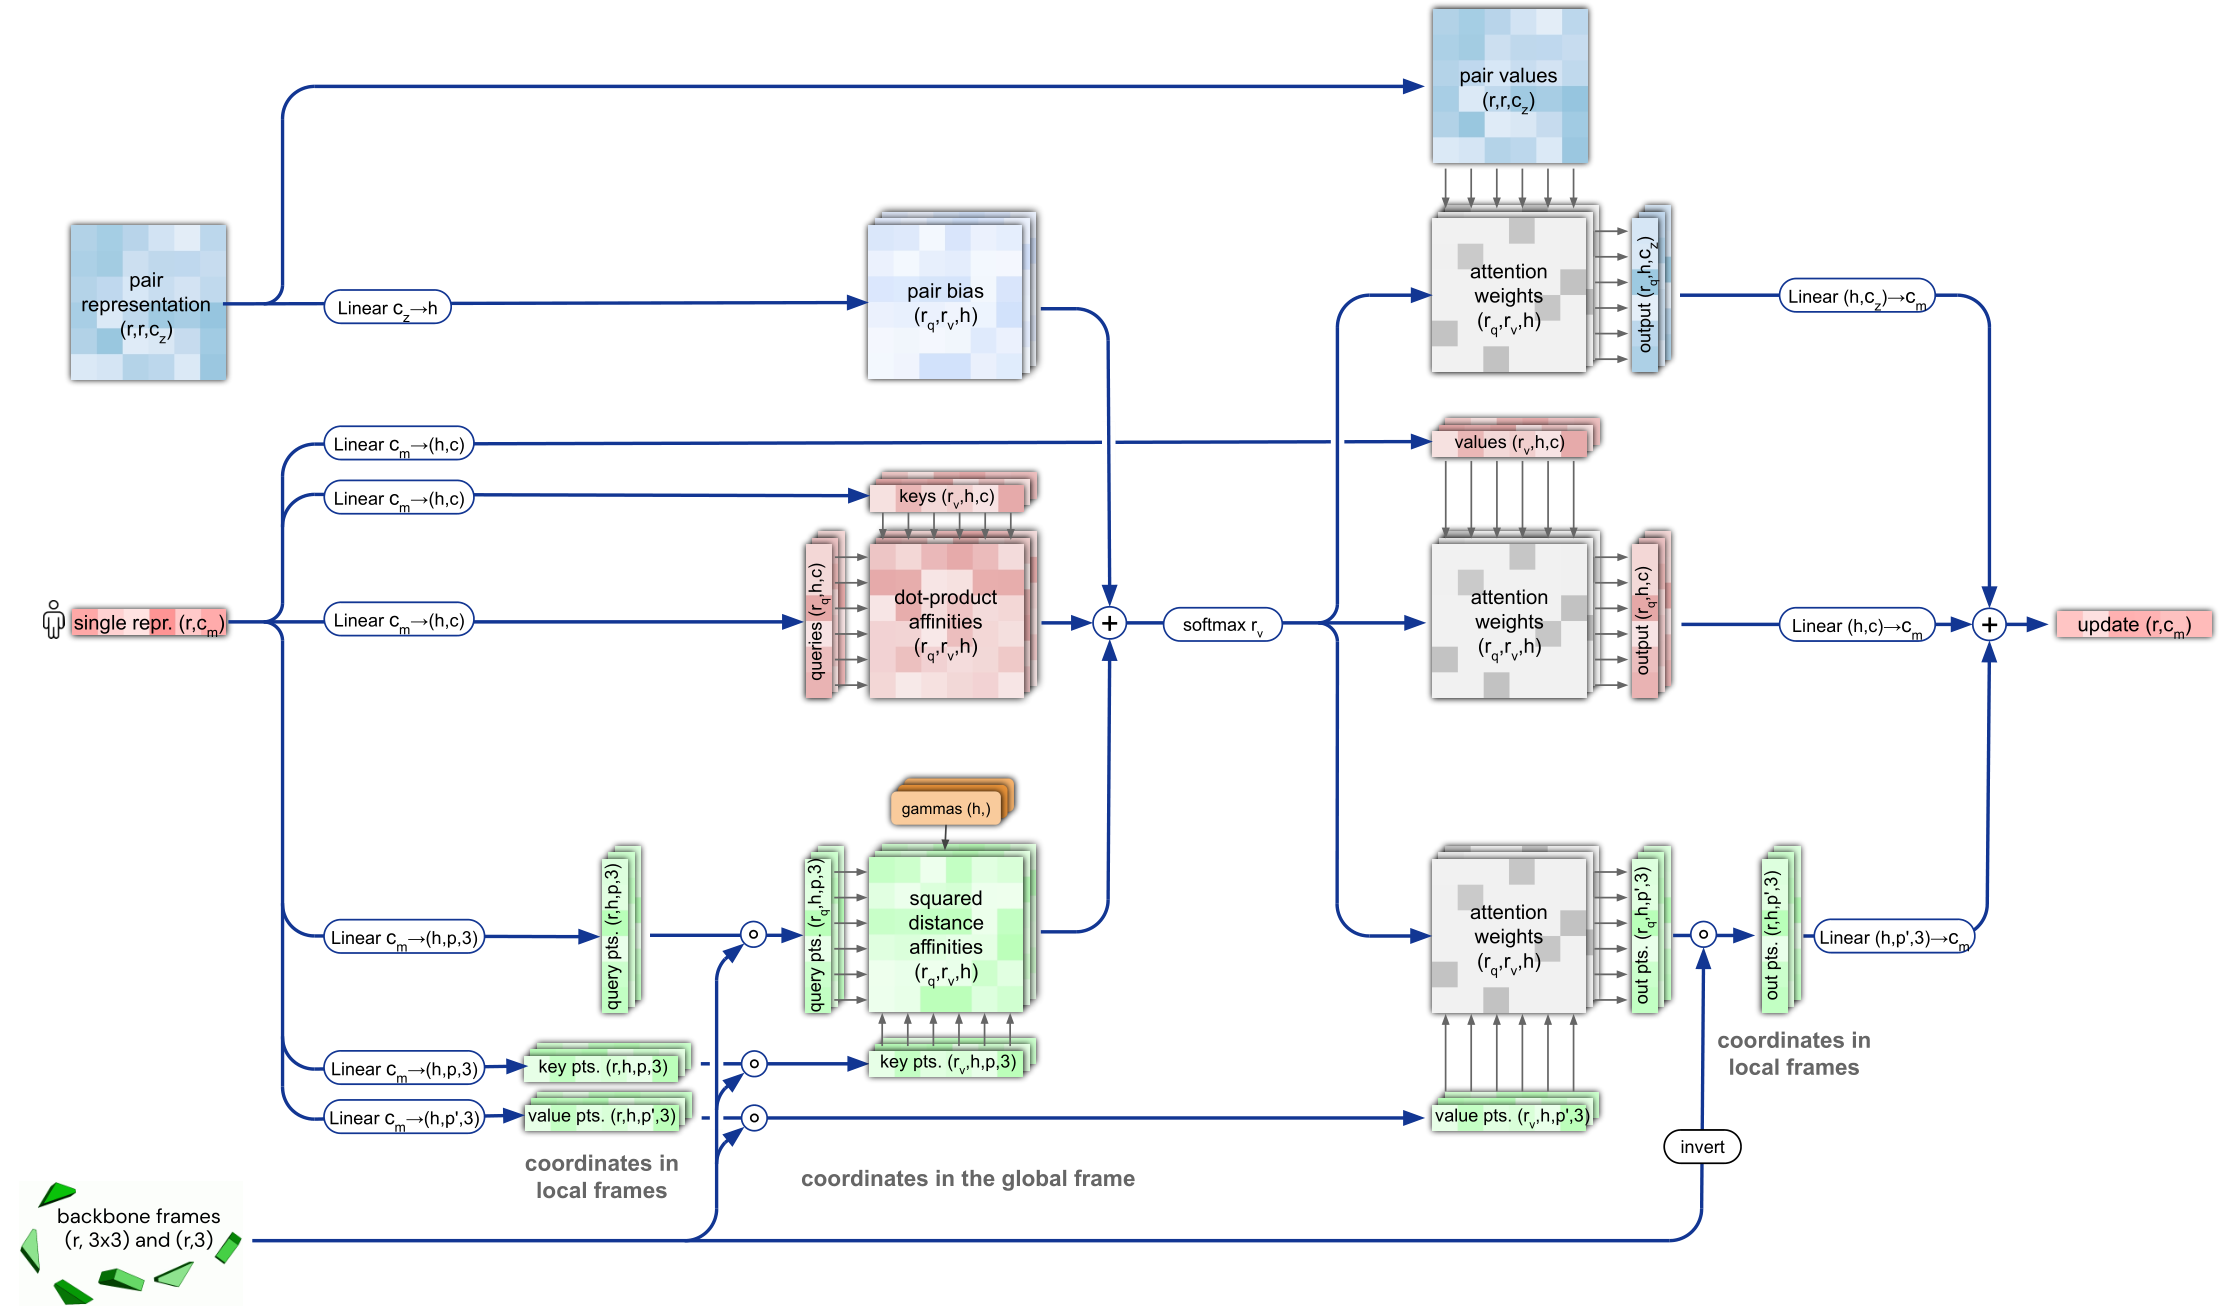
\includegraphics[width=.9\linewidth]{./imgs/ipa.png}
\end{center}
\end{frame}

\begin{frame}[label={sec:org2e83edb}]{Structure Module: Algorithm Part 1 \cite{jumperHighlyAccurateProtein2021}}
\begin{center}
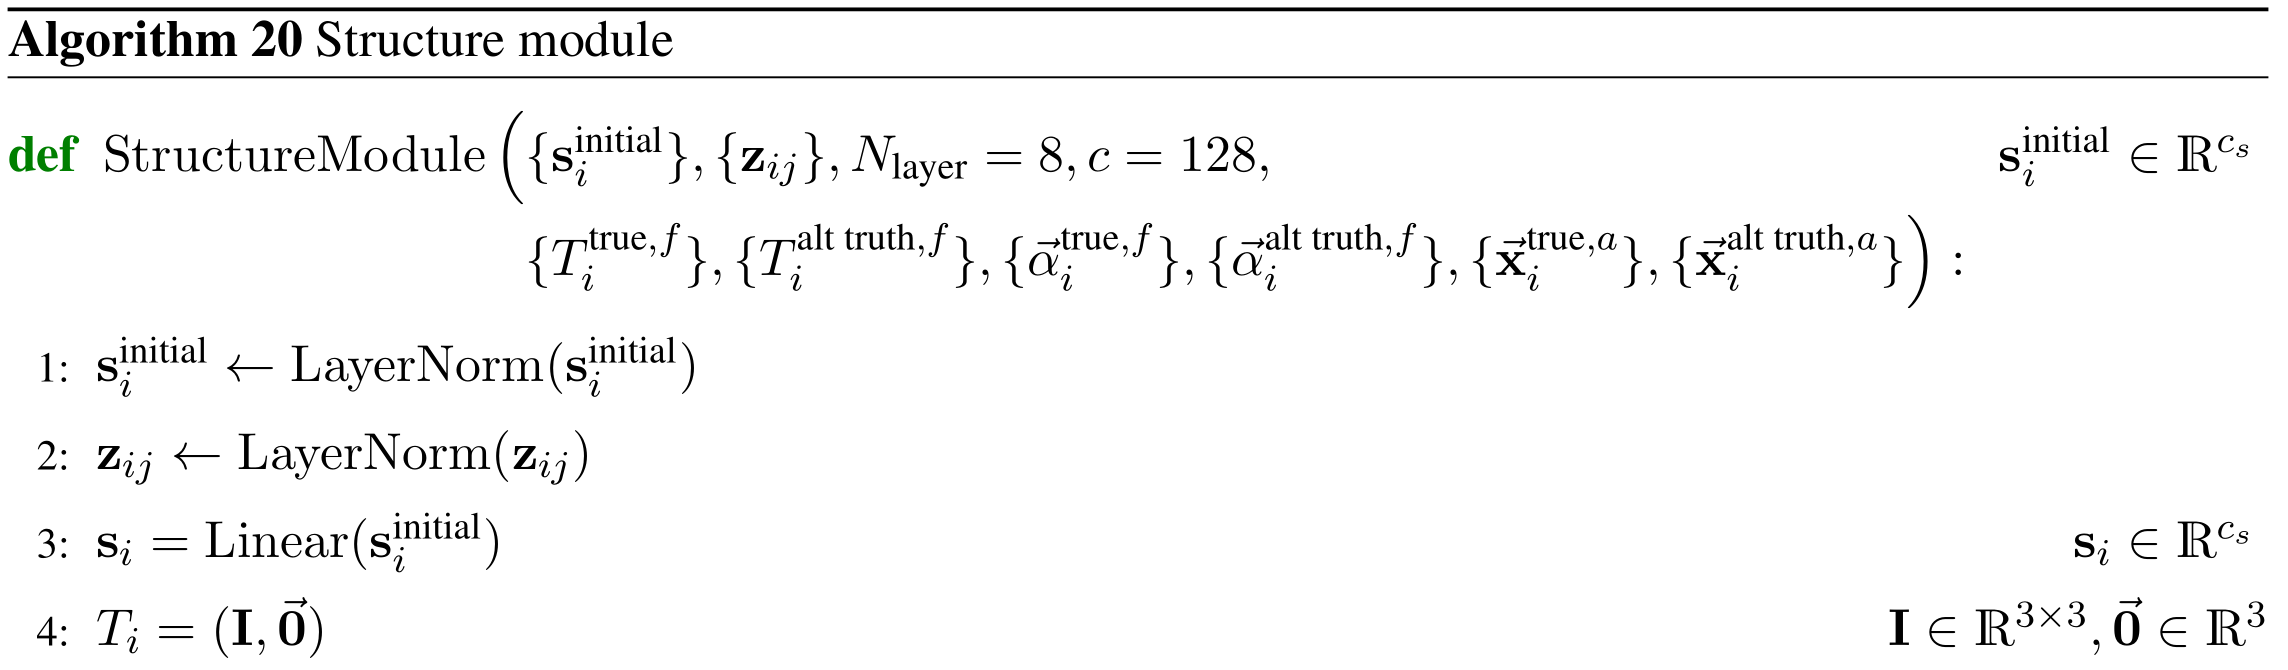
\includegraphics[width=.9\linewidth]{./imgs/algo20-part1.png}
\end{center}
\end{frame}

\begin{frame}[label={sec:orgb2d0717}]{Structure Module: Algorithm Part 2 \cite{jumperHighlyAccurateProtein2021}}
\begin{center}
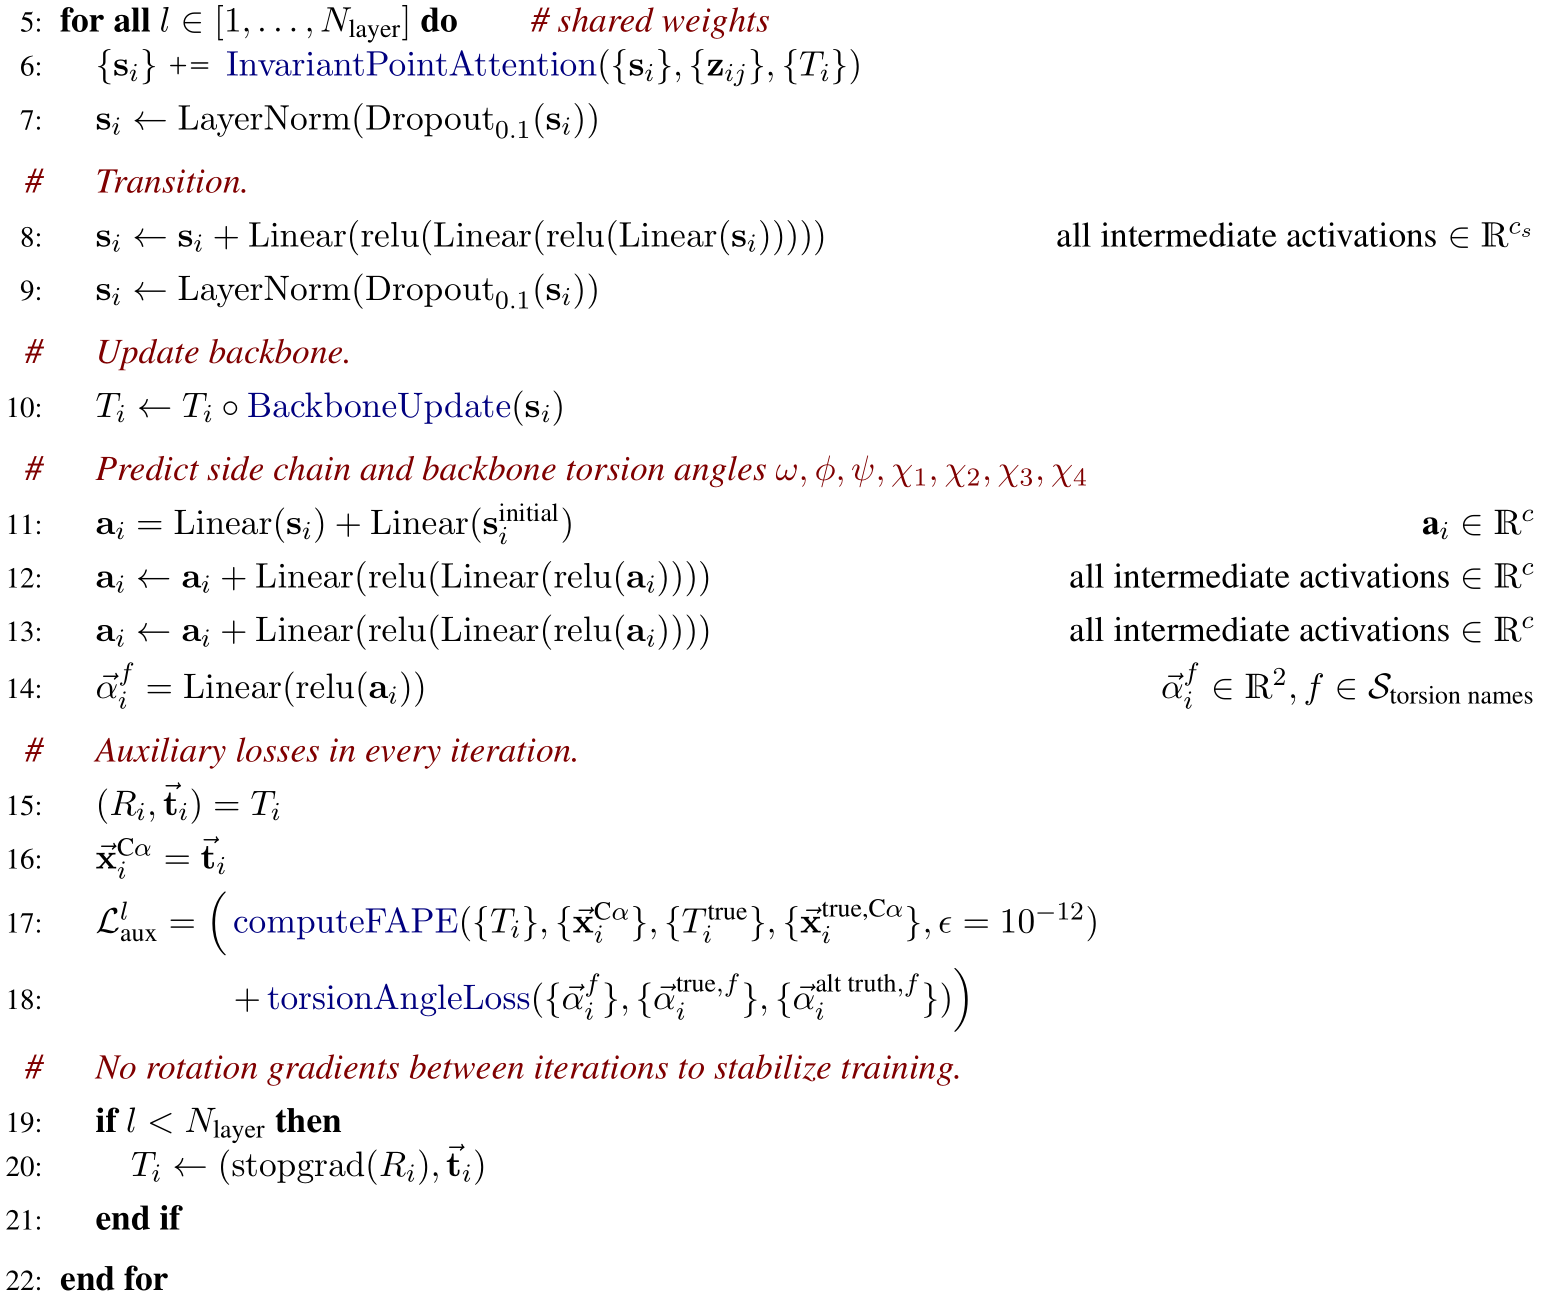
\includegraphics[width=.9\linewidth]{./imgs/algo20-part2.png}
\end{center}
\end{frame}

\begin{frame}[label={sec:orgf5bfc43}]{Structure Module: Algorithm Part 3 \cite{jumperHighlyAccurateProtein2021}}
\begin{center}
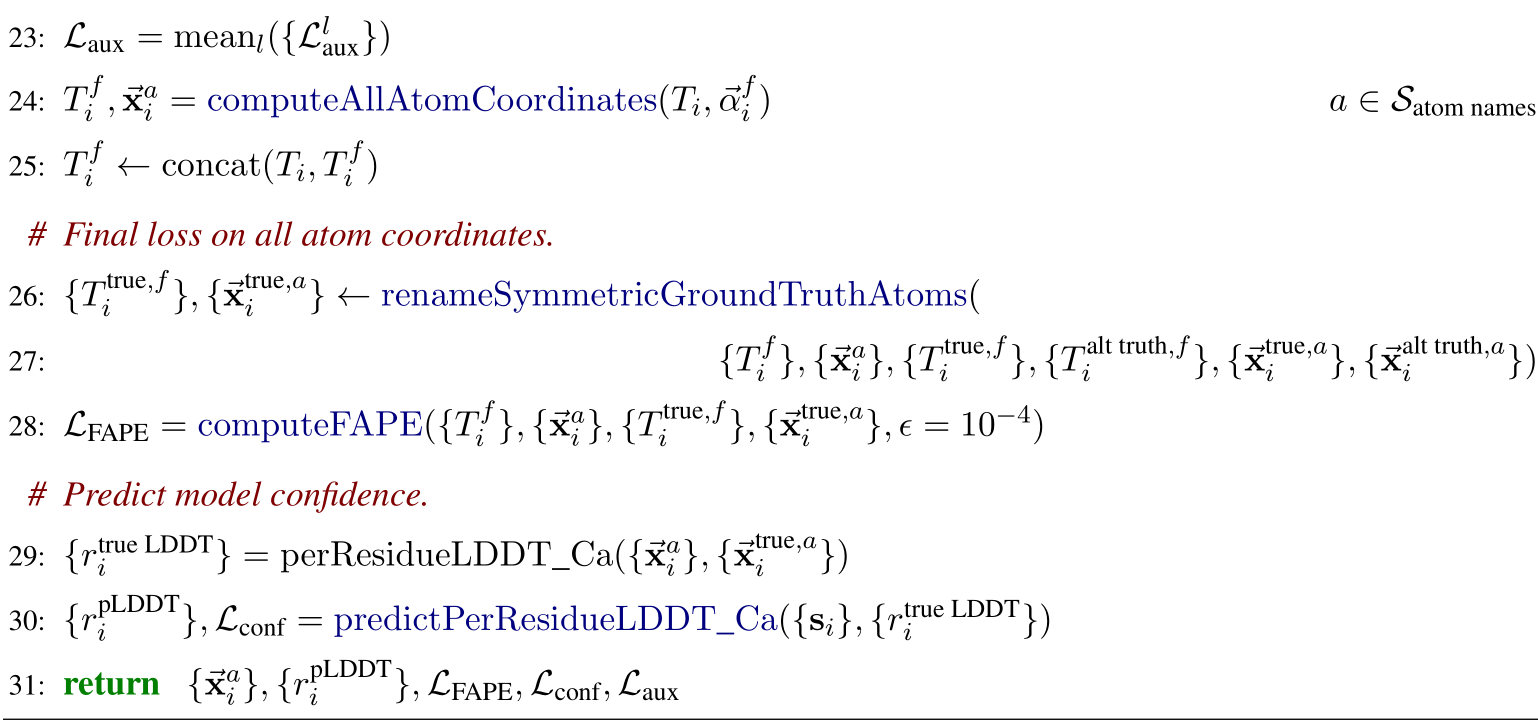
\includegraphics[width=.9\linewidth]{./imgs/algo20-part3.png}
\end{center}
\end{frame}

\subsection*{Final}
\label{sec:orge63b1f1}
\begin{frame}[label={sec:org68597aa}]{Loss Functions  \cite{jumperHighlyAccurateProtein2021}}
\begin{center}
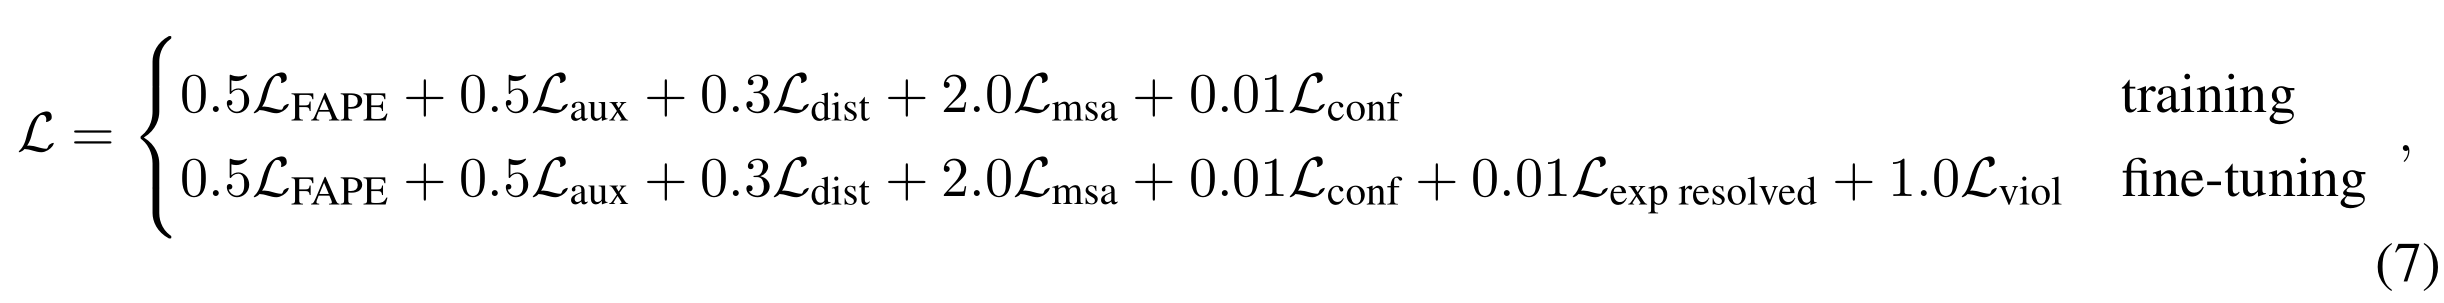
\includegraphics[width=.9\linewidth]{./imgs/loss-eq.png}
\end{center}

\begin{itemize}
\item weighted sum
\item weighted to reduce importance of short sequences
\end{itemize}
\end{frame}

\begin{frame}[label={sec:org7acd076}]{Loss Functions \& Auxillary Heads \cite{jumperHighlyAccurateProtein2021}}
\begin{enumerate}
\item Side chain and backbone torsion angle loss
\item Frame aligned point error (FAPE)
\begin{itemize}
\item Configurations with FAPE(X,Y) = 0
\item Metric properties of FAPE
\end{itemize}
\item Chiral properties of AlphaFold and its loss
\item Model confidence prediction (pLDDT)
\item TM-score prediction
\item Distogram prediction
\item Masked MSA prediction
\item "Experimentally resolved" prediction
\item Structural violations
\end{enumerate}
\end{frame}

\begin{frame}[label={sec:org3486362}]{Loss Functions: FAPE}
\begin{center}
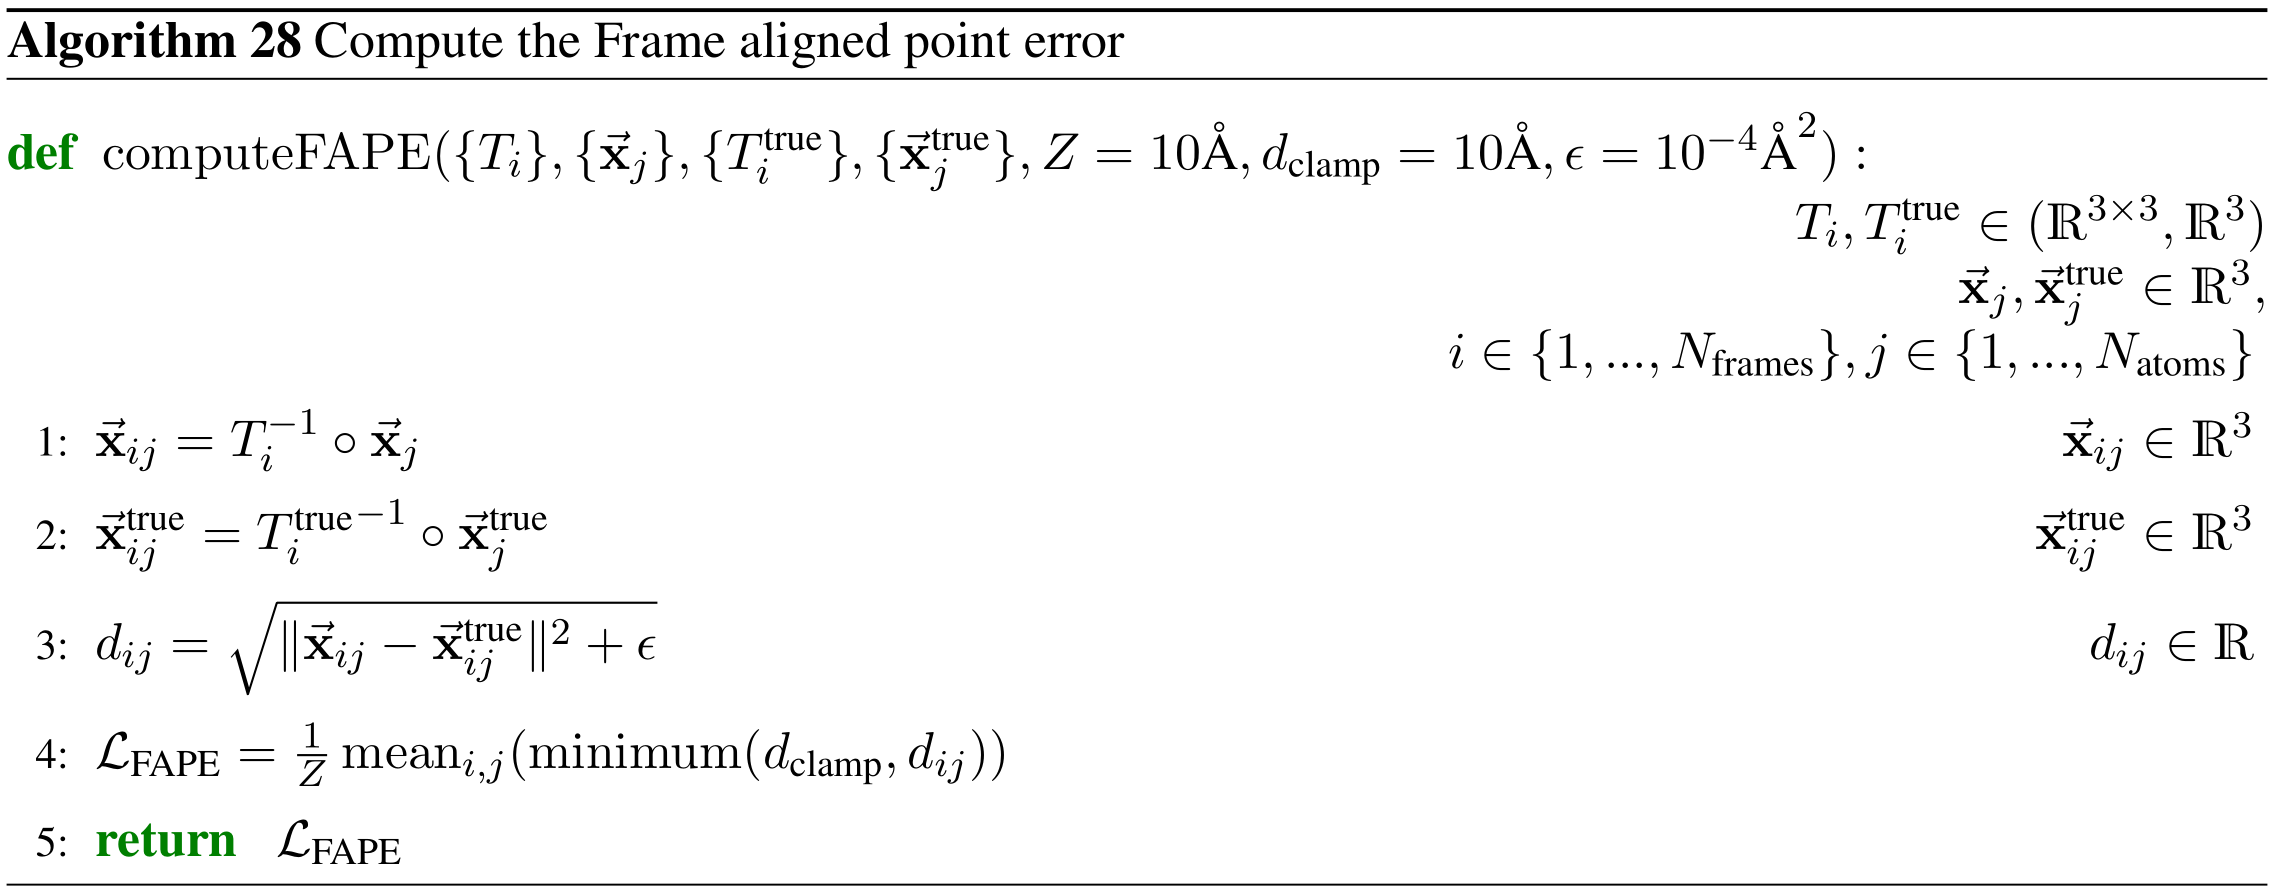
\includegraphics[width=.9\linewidth]{./imgs/fape-algo.png}
\end{center}
\cite{jumperHighlyAccurateProtein2021}

\begin{itemize}
\item Variation of commonly used root-mean-squared deviation (RMSD) of atomic positions
\item not invariant to reflections, preventing proteins of the wrong chirality. \cite{rubieraAlphaFoldHereWhat}, \cite{jumperHighlyAccurateProtein2021}
\end{itemize}
\end{frame}

\section*{AlphaFold Inference}
\label{sec:org9bad96d}
\begin{frame}[label={sec:orgaec583a}]{AlphaFold Inference \cite{jumperHighlyAccurateProtein2021}}
\begin{itemize}
\item AlphaFold receives input features derived from:
\begin{itemize}
\item the amino-acid sequence
\item MSA
\item templates (see subsubsection 1.2.9)
\end{itemize}
\item outputs features:
\begin{itemize}
\item atom coordinates
\item the distogram
\item per-residue confidence scores.
\end{itemize}
\item Recycling x3
\begin{itemize}
\item initial recycled inputs are zero
\end{itemize}
\end{itemize}

Algorithm 2 outlines the main steps (see also Fig 1e and the corresponding description in the main article).
\end{frame}

\begin{frame}[label={sec:org3d7da98}]{AlphaFold Training \cite{jumperHighlyAccurateProtein2021}}
\begin{center}
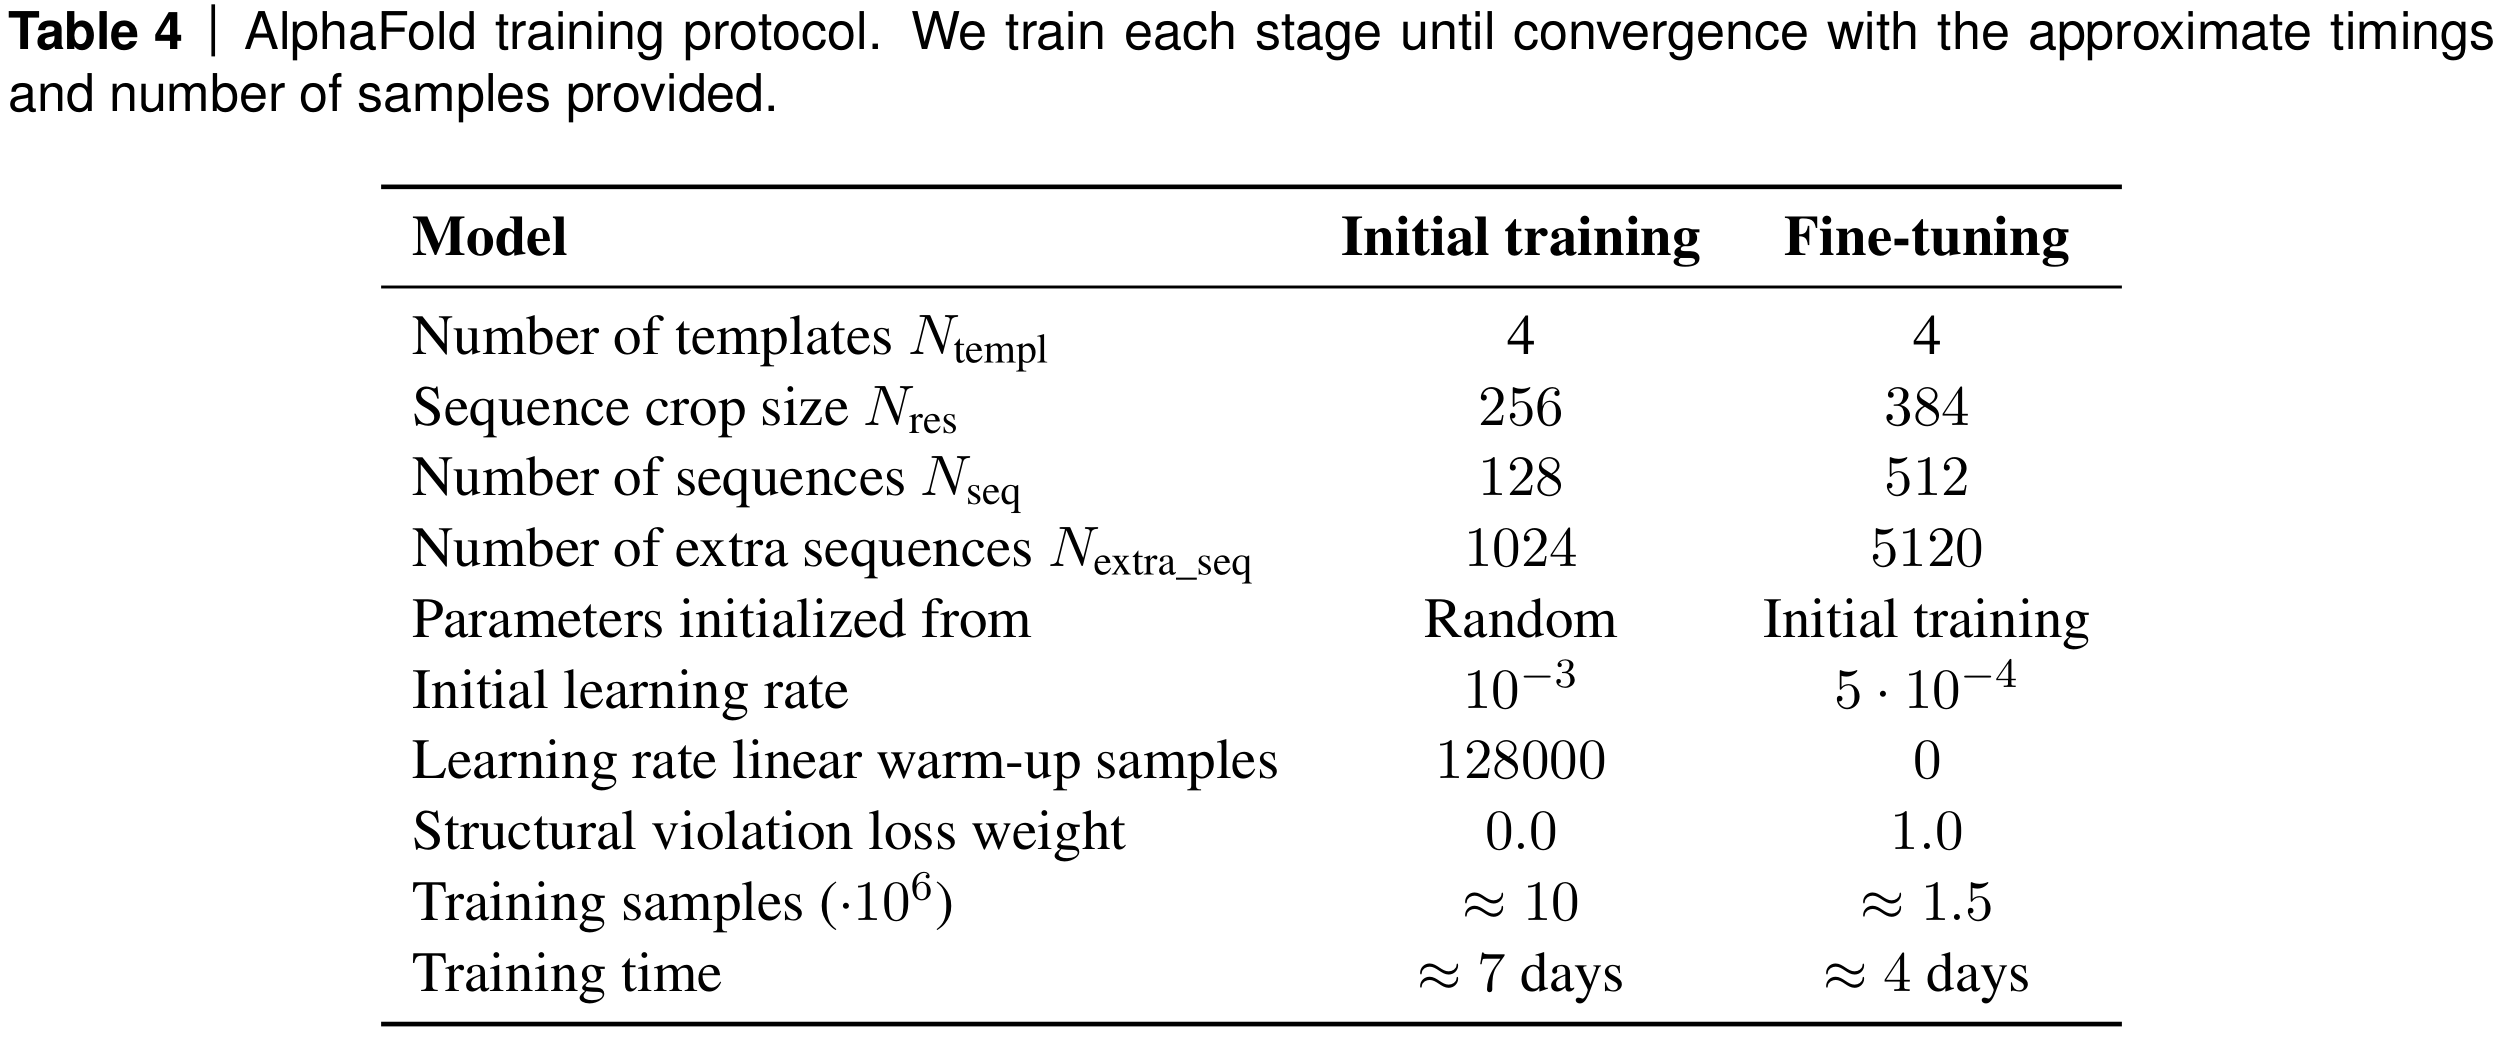
\includegraphics[width=.9\linewidth]{./imgs/af-training-table.png}
\end{center}
\end{frame}

\section*{Results}
\label{sec:org26fc1f6}
\begin{frame}[label={sec:orgdf093a1}]{Results \cite{jumperHighlyAccurateProtein2021}}
They did well
\end{frame}

\begin{frame}[label={sec:org6d024dd}]{Results \cite{jumperHighlyAccurateProtein2021}}
They did well
\end{frame}

\begin{frame}[label={sec:org3558b44}]{Results: Positional Encodings \cite{jumperHighlyAccurateProtein2021}}
\end{frame}

\begin{frame}[label={sec:org8bfe2c5}]{Novel Folds}
They did well
\end{frame}

\begin{frame}[label={sec:org0309b4b}]{Ablation Studies \cite{jumperHighlyAccurateProtein2021}}
Baseline for all ablation models: Full model without noisy-student self-attention  
Ablations:
\begin{enumerate}
\item With noisy-student self-distillation training
\item No templates
\item No raw MSA (use MSA pairwise frequencies)
\item No triangles, biasing, or gating (use axial attention)
\item No recycling
\item No IPA (use direct projection)
\item No invariant IPA \& no recycling
\item No end-to-end structure gradients (keep auxiliary heads)
\item No auxiliary distogram head
\item No auxiliary masked MSA head
\end{enumerate}
\end{frame}

\begin{frame}[label={sec:org832561a}]{Network Probing \cite{jumperHighlyAccurateProtein2021}}
todo
\end{frame}

\begin{frame}[label={sec:orgc7aea41}]{Attention Visualization \cite{jumperHighlyAccurateProtein2021}}
todo
\end{frame}

\section*{Algorithms}
\label{sec:org070459f}
\begin{frame}[label={sec:org557465e}]{Algorithm 24 Compute all atom coordinates \cite{jumperHighlyAccurateProtein2021}}
\begin{center}
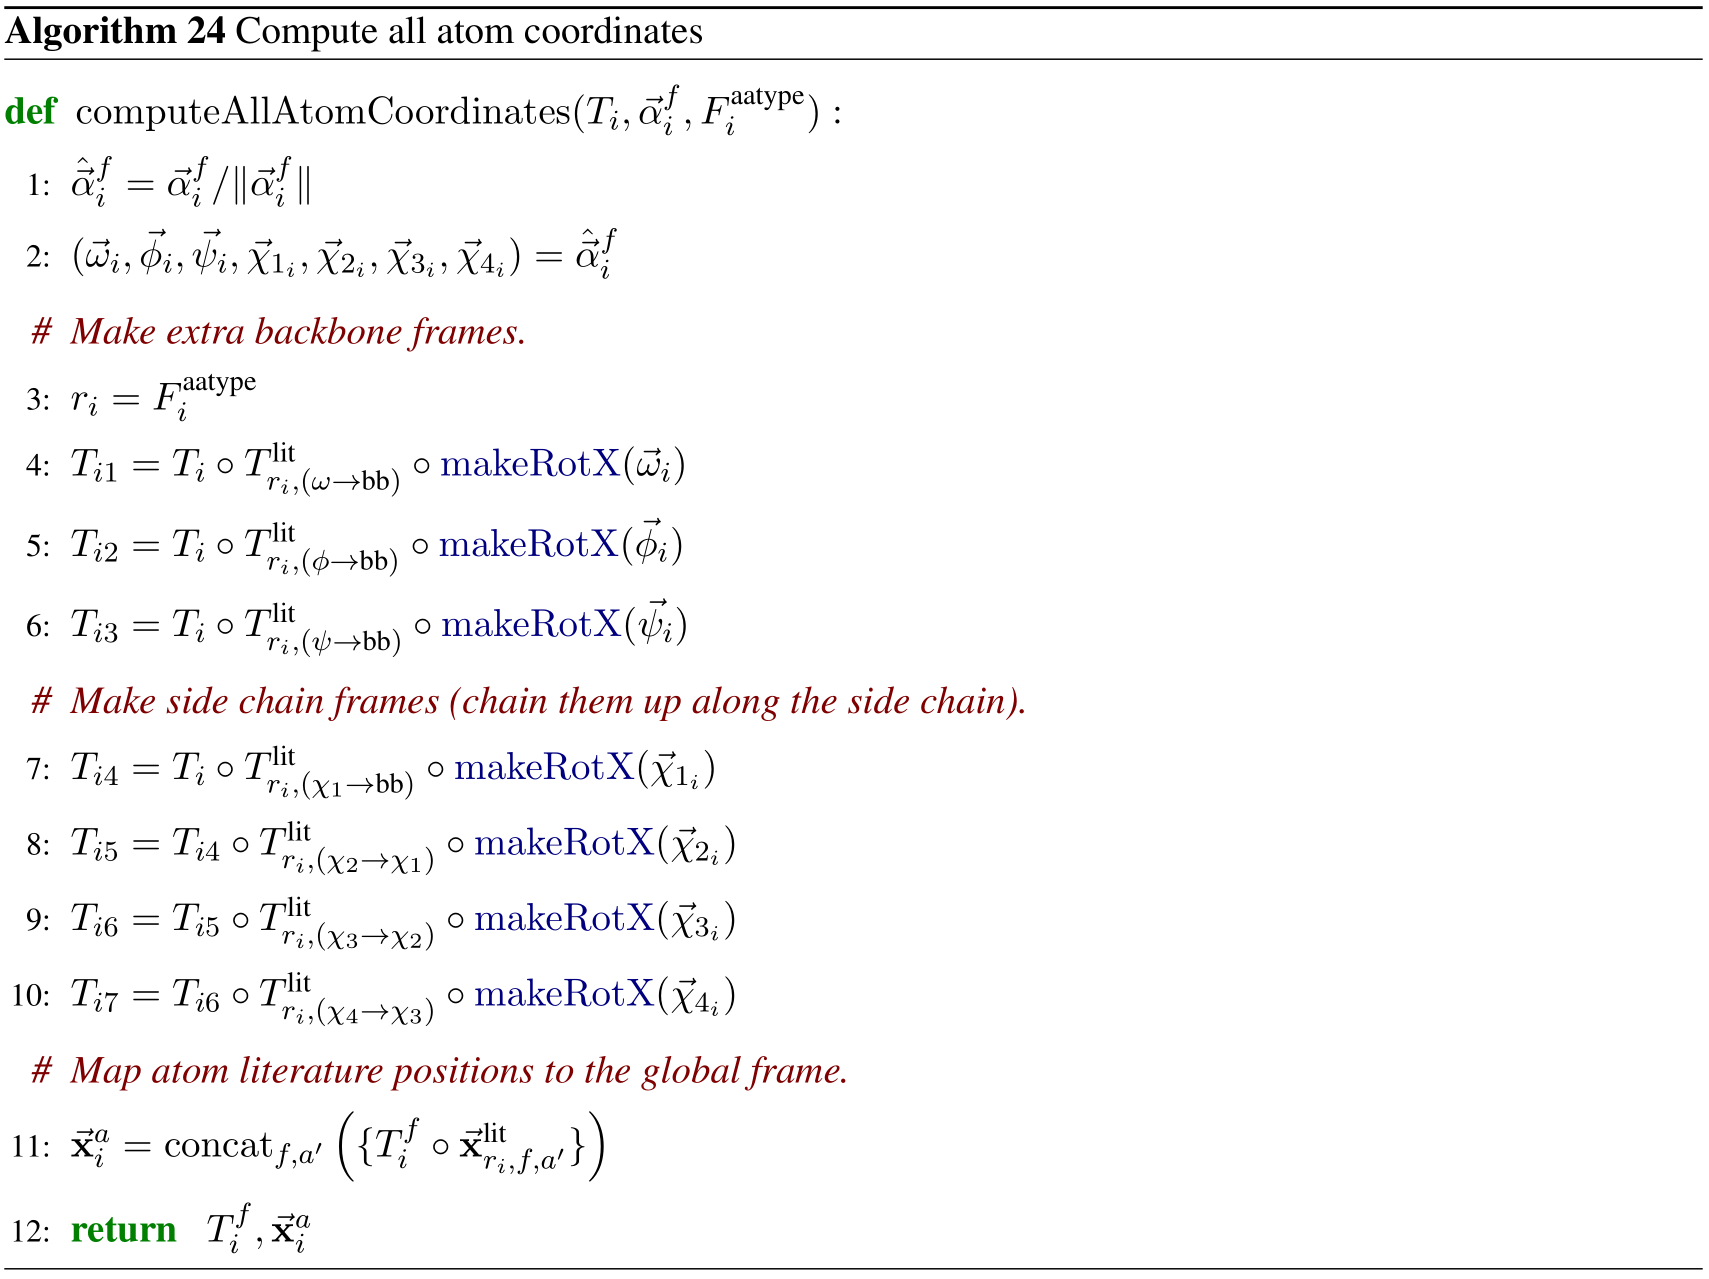
\includegraphics[width=.9\linewidth]{./imgs/all-atom-coords-algo.png}
\end{center}
\end{frame}
\begin{frame}[label={sec:org0170fe9}]{Algorithm 23 Backbone update \cite{jumperHighlyAccurateProtein2021}}
\begin{center}
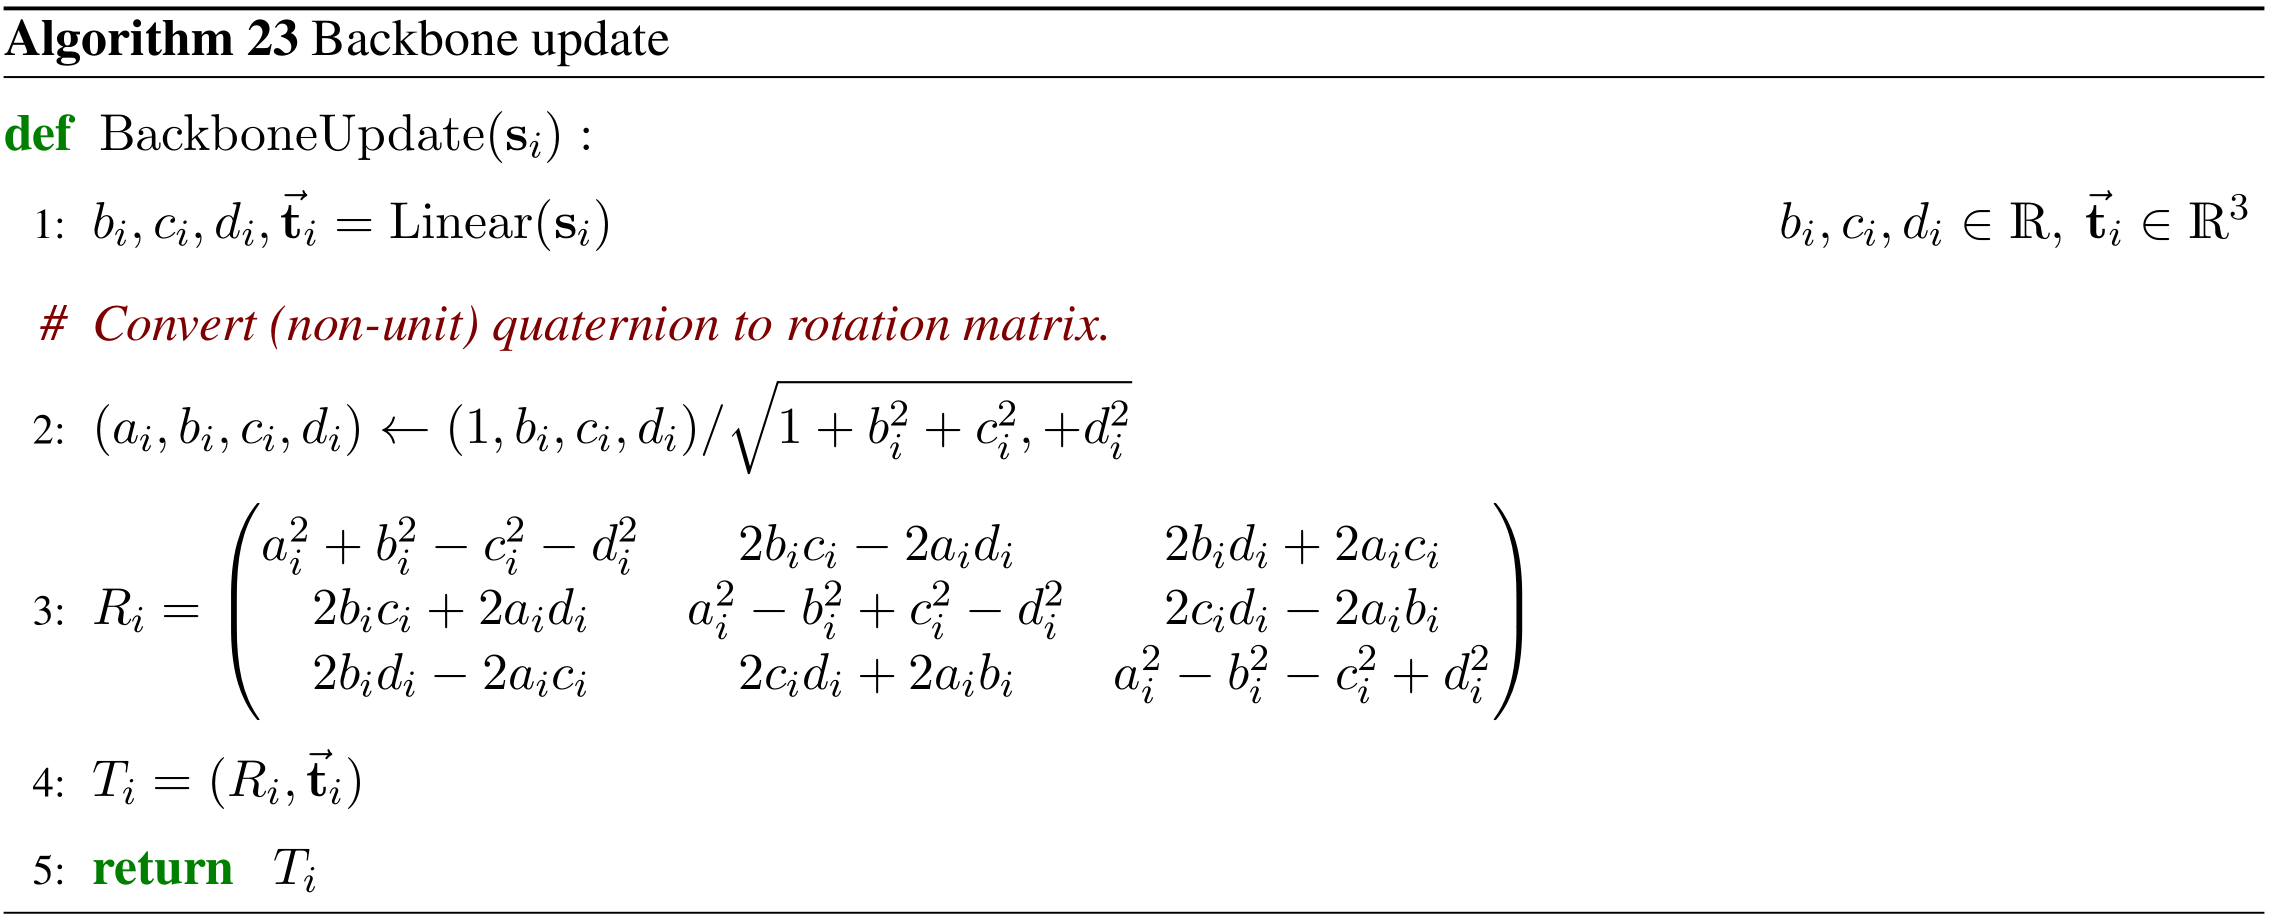
\includegraphics[width=.9\linewidth]{./imgs/backbone-update-algo.png}
\end{center}
\end{frame}
\begin{frame}[label={sec:org8eba1c7}]{Algorithm 29 Predict model confidence pLDDT \cite{jumperHighlyAccurateProtein2021}}
\begin{center}
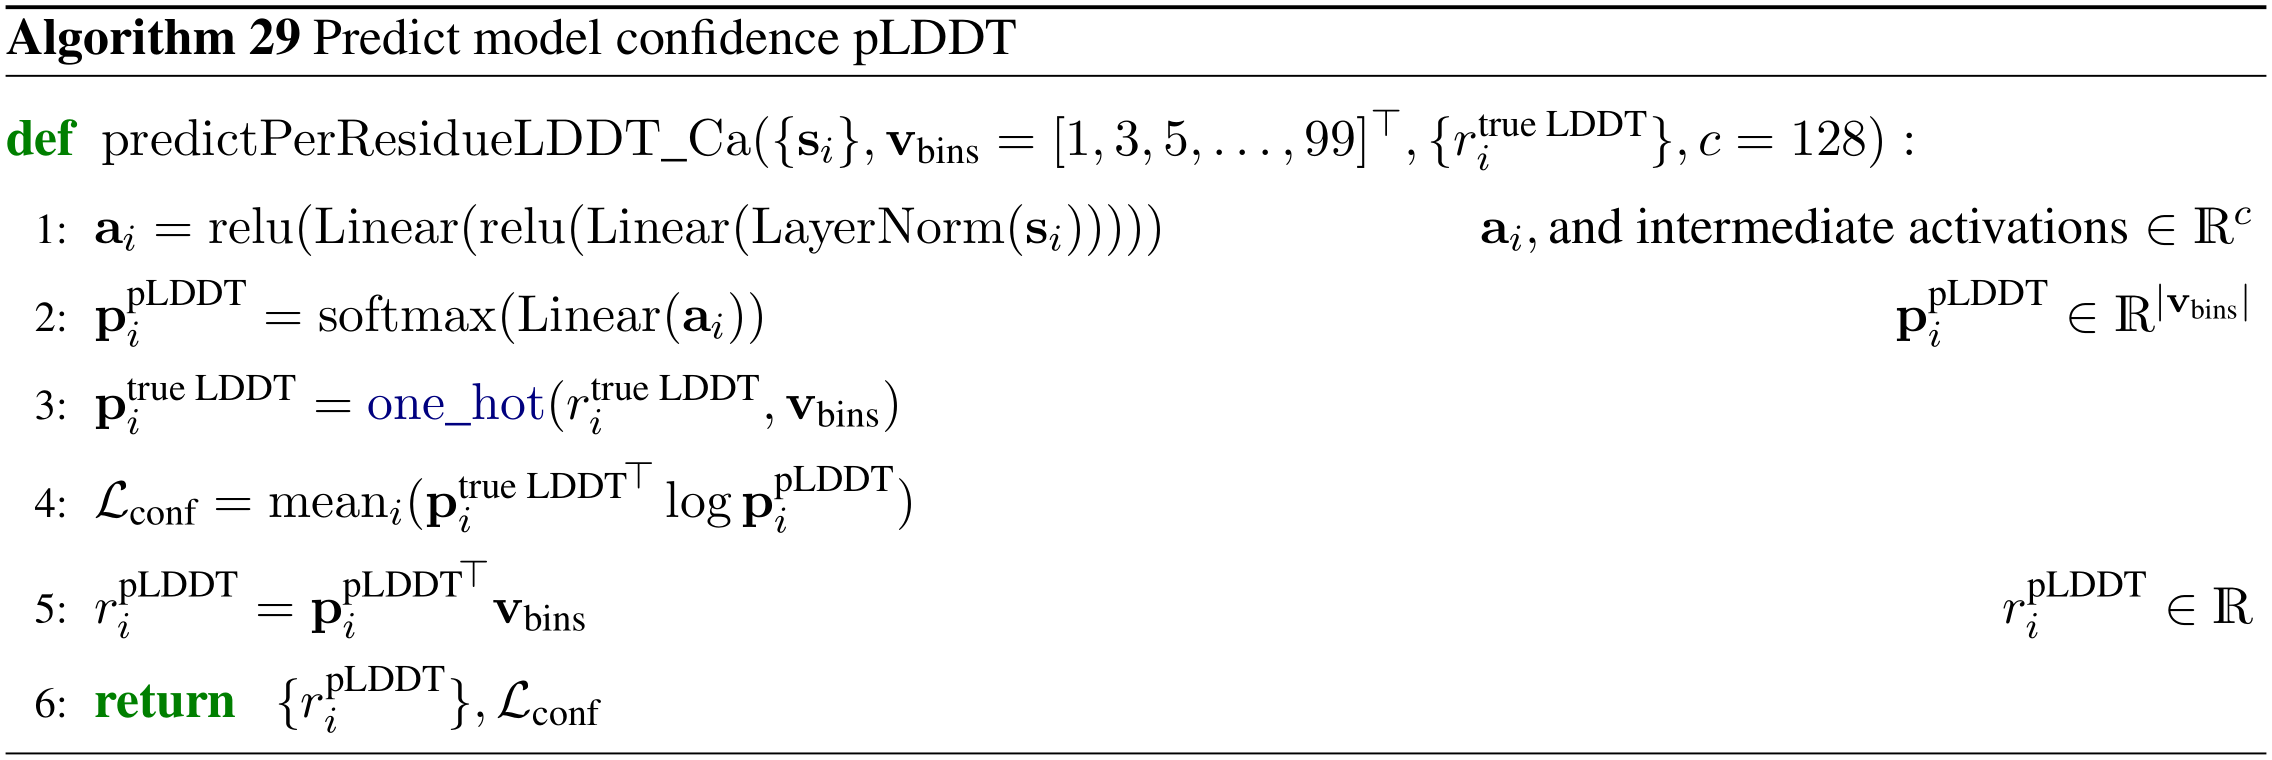
\includegraphics[width=.9\linewidth]{./imgs/confidence-pLDDT-algo29.png}
\end{center}
\end{frame}
\begin{frame}[label={sec:org963bd98}]{Distograms \cite{jumperHighlyAccurateProtein2021}}
\begin{center}
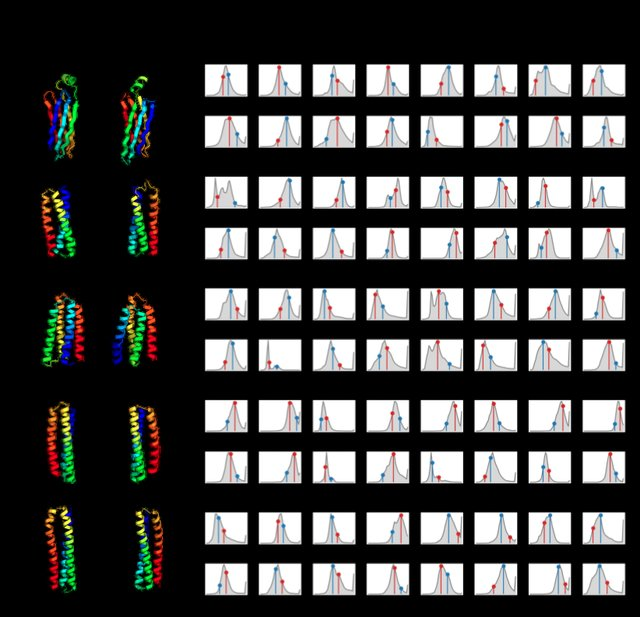
\includegraphics[height=\textheight]{./imgs/Examples-of-distograms-from-trRosetta.jpg}
\end{center}
\end{frame}
\begin{frame}[label={sec:orgaa37153}]{Algorithm 31 Generic recycling training procedure \cite{jumperHighlyAccurateProtein2021}}
\begin{center}
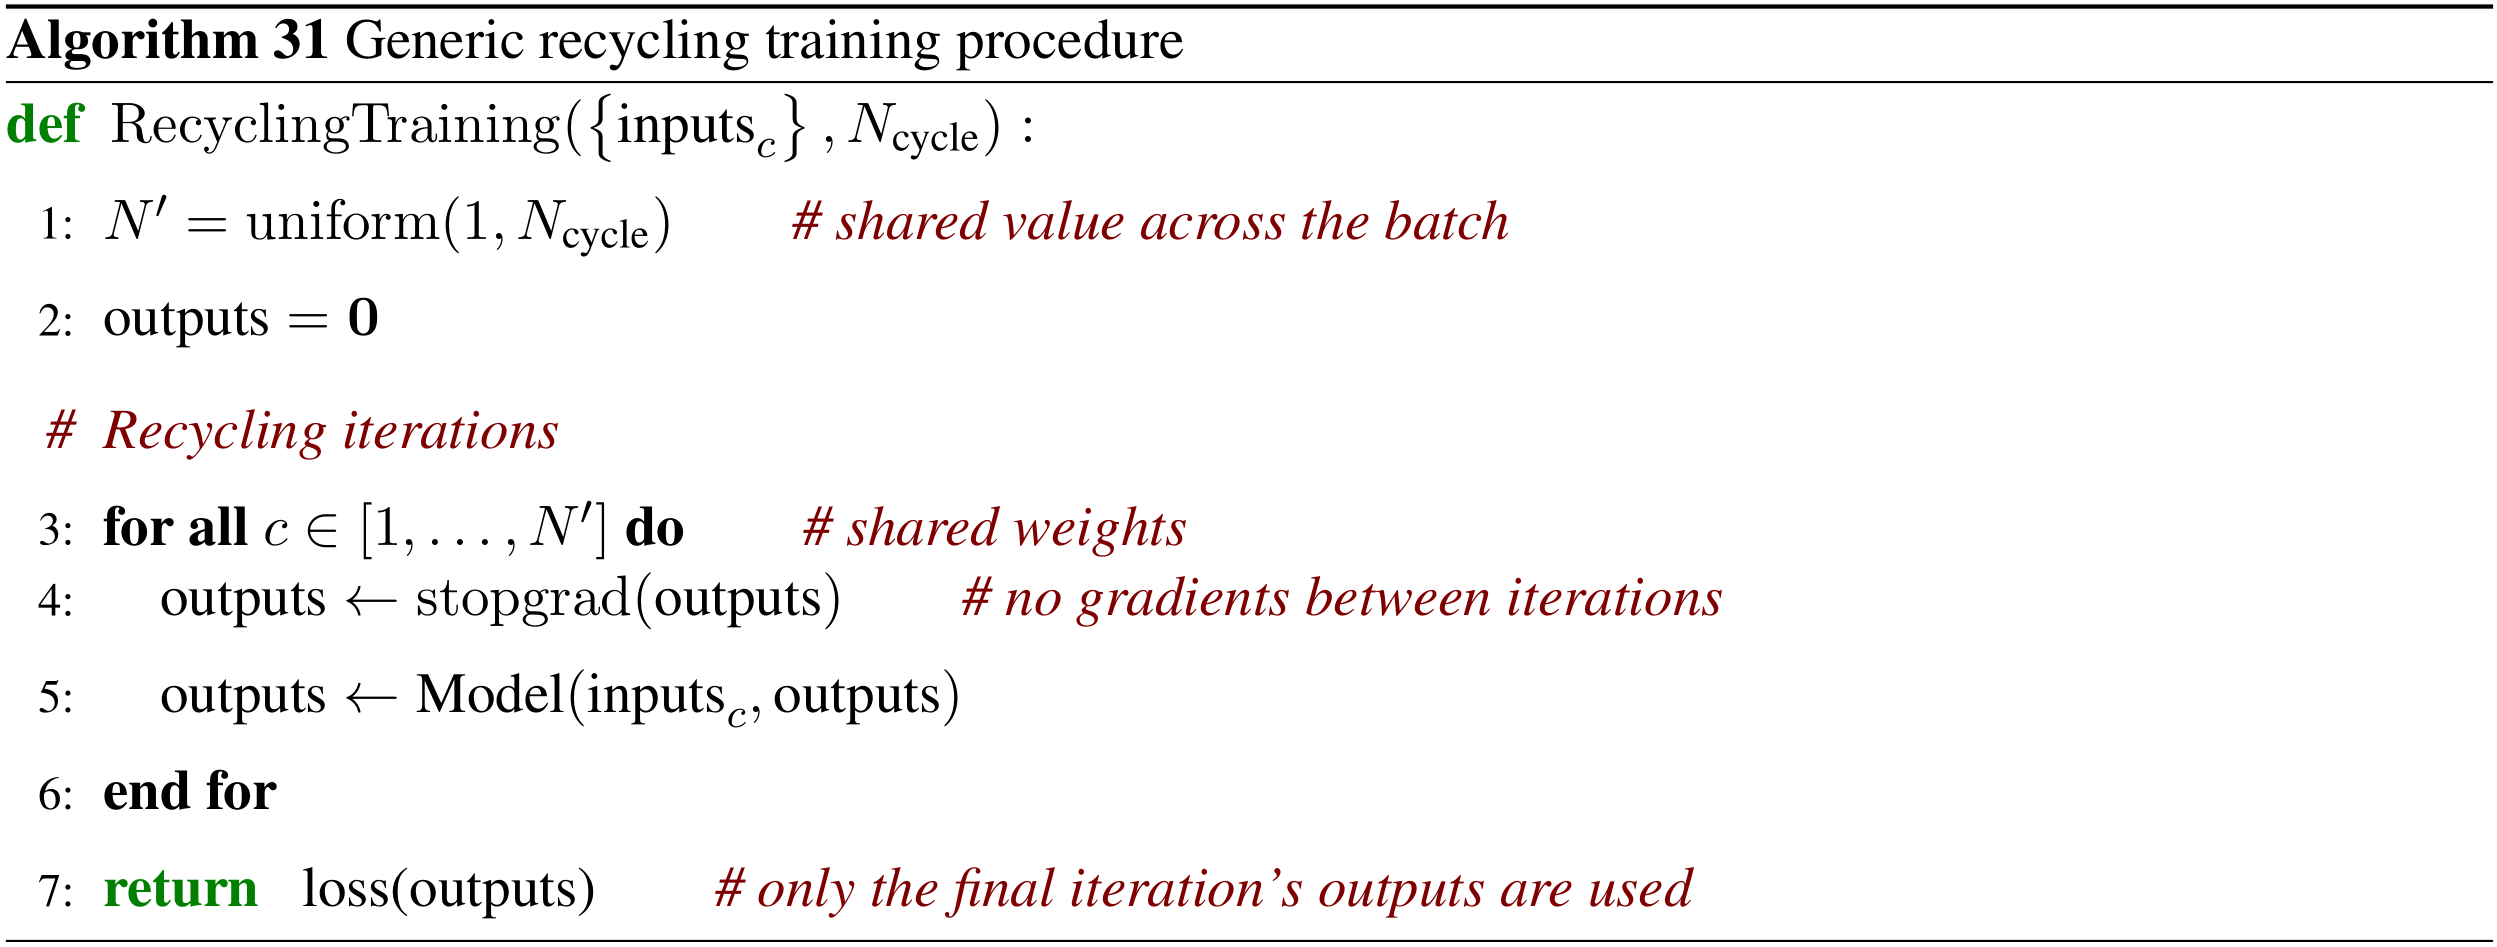
\includegraphics[width=.9\linewidth]{./imgs/generic-recycling-algo31.png}
\end{center}
\end{frame}
\begin{frame}[label={sec:orgbb2ef35}]{Algorithm 30 Generic recycling inference procedure \cite{jumperHighlyAccurateProtein2021}}
\begin{center}
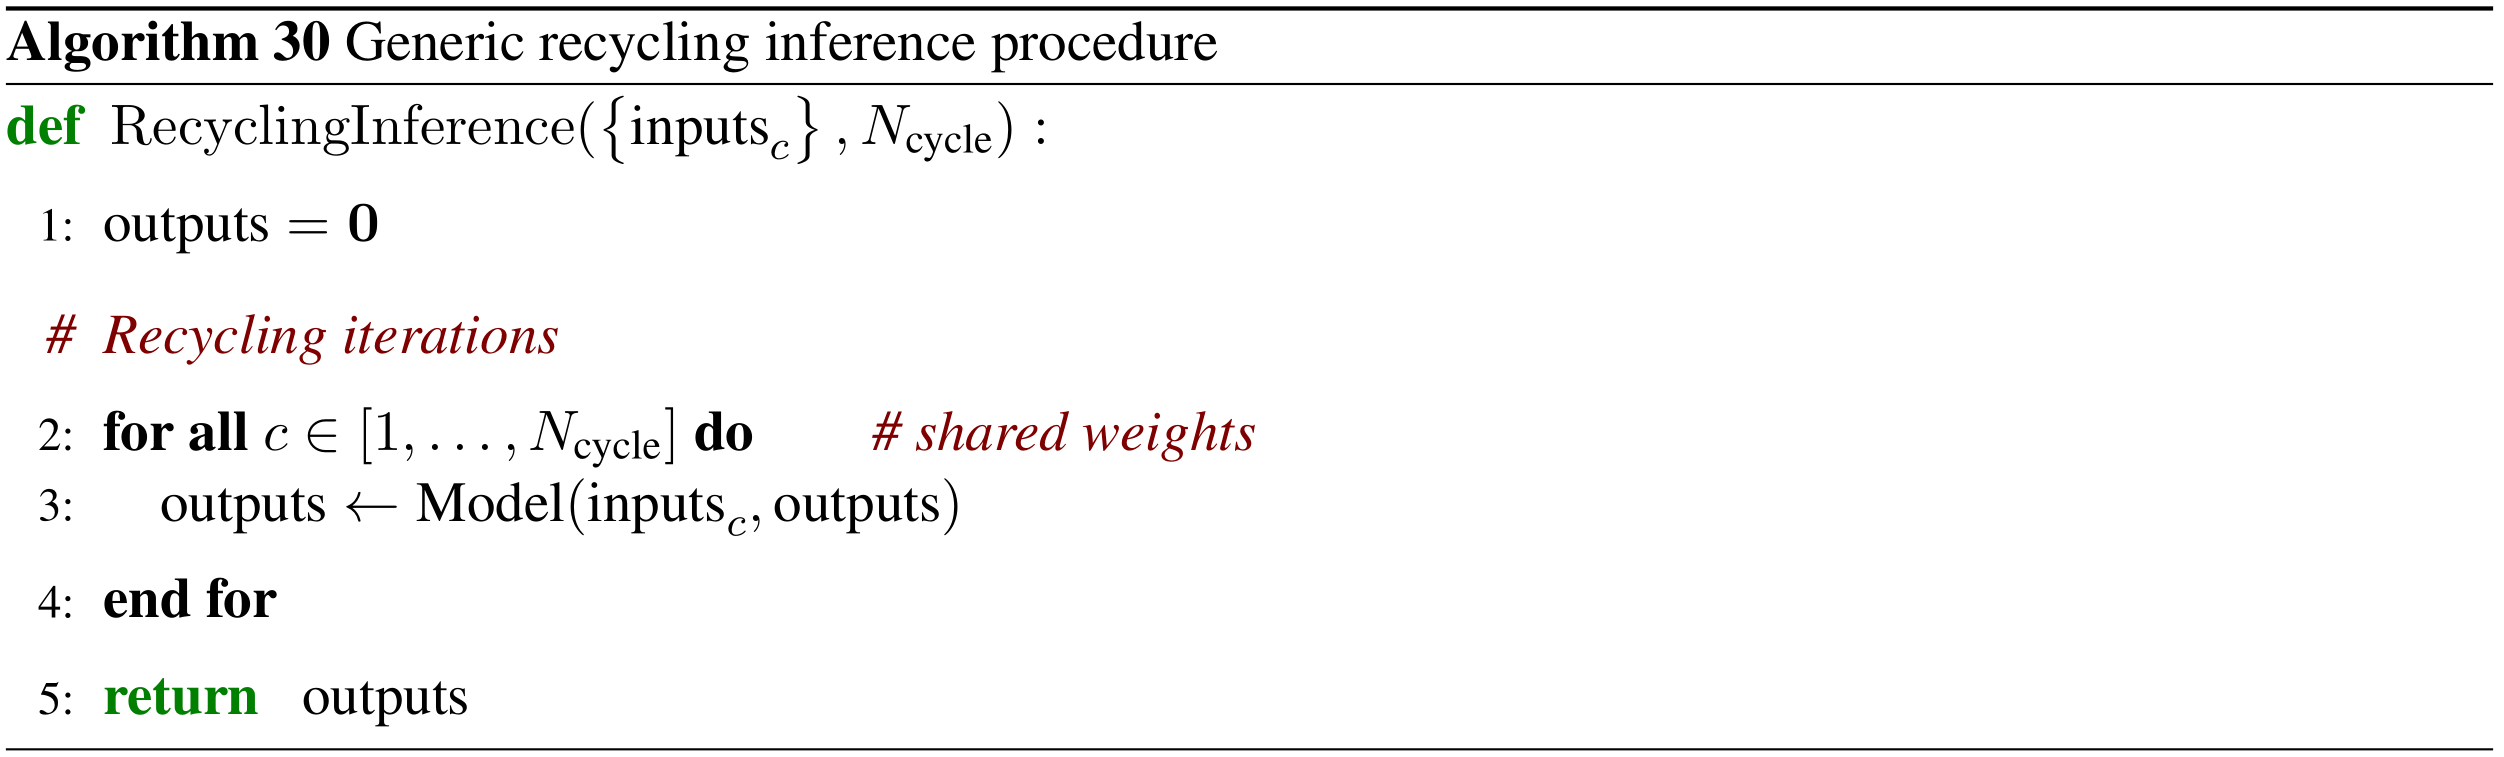
\includegraphics[width=.9\linewidth]{./imgs/recycling-algo30.png}
\end{center}
\end{frame}
\begin{frame}[label={sec:org550ce4a}]{Algorithm 32 Embedding of evoformer and structure module outputs for recycling \cite{jumperHighlyAccurateProtein2021}}
\begin{center}
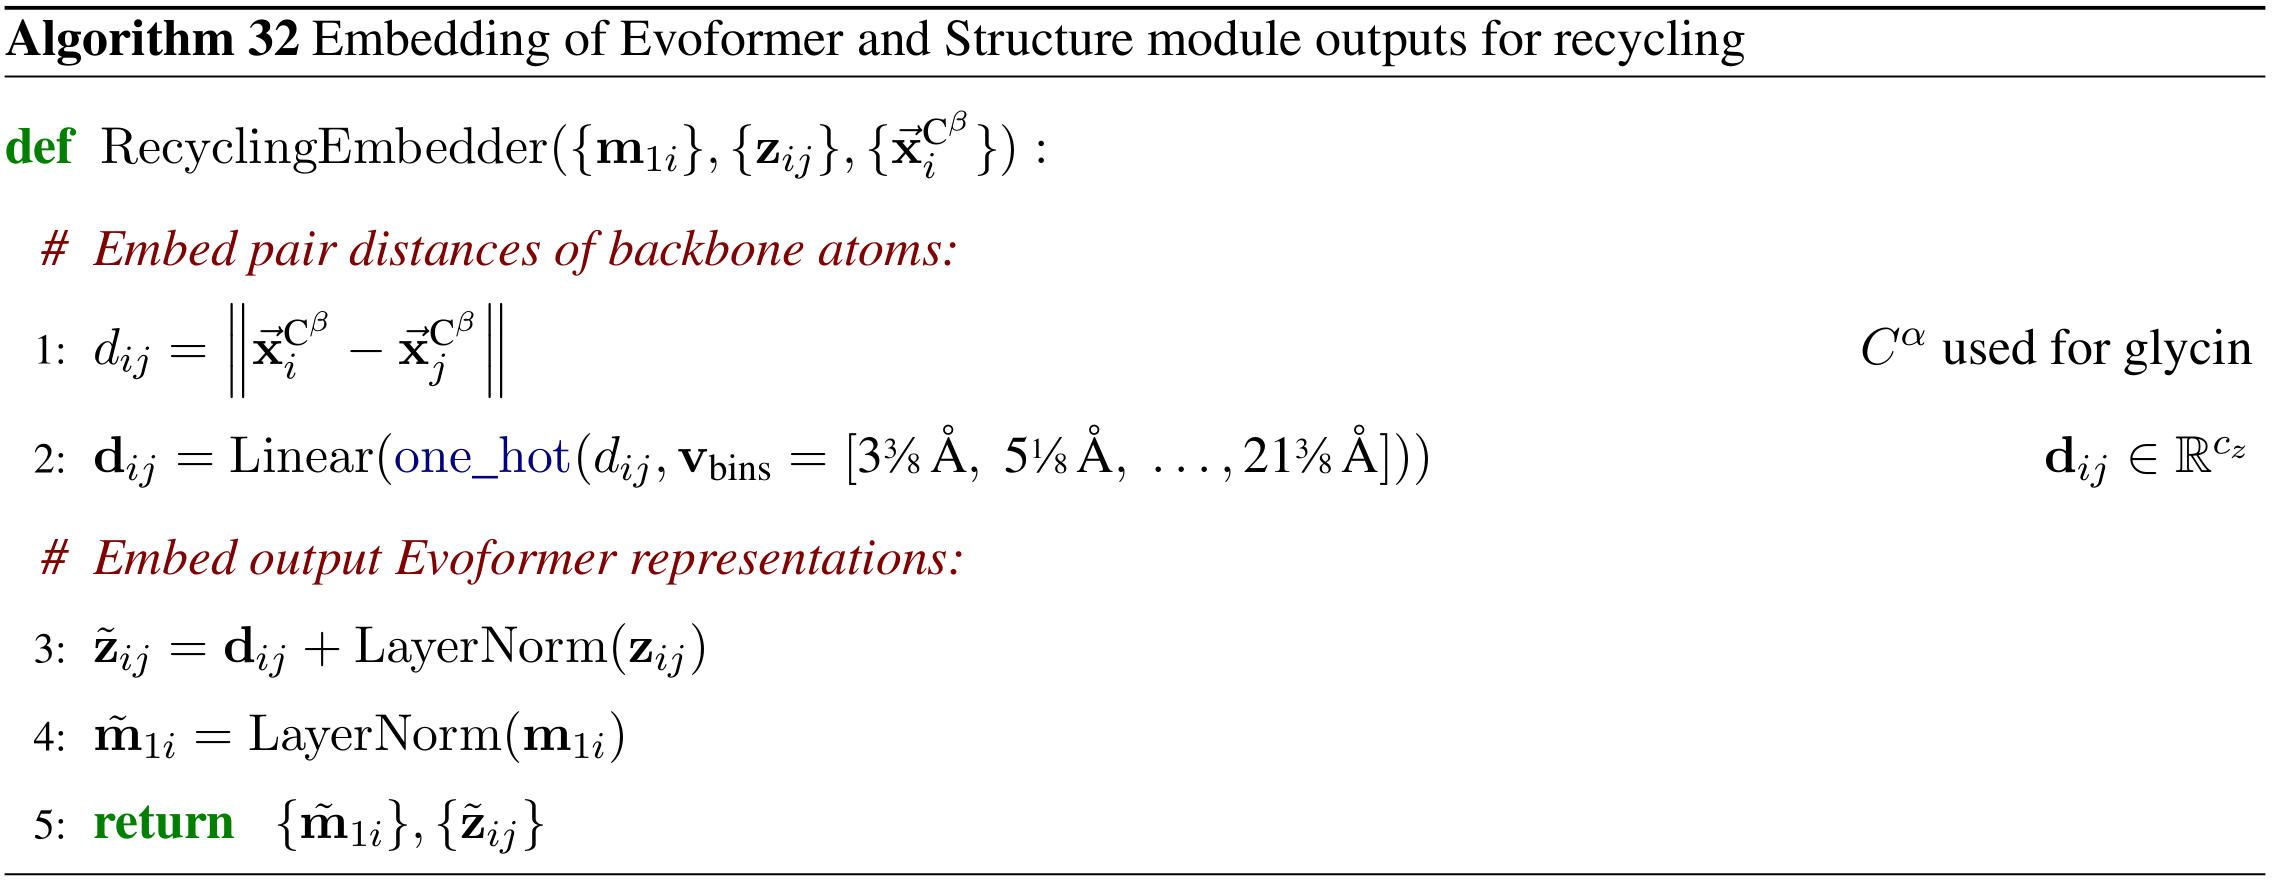
\includegraphics[width=.9\linewidth]{./imgs/recycling-embedding-algo32.png}
\end{center}
\end{frame}
\begin{frame}[label={sec:org71dc79c}]{Algorithm 26 Rename symmetric ground truth atoms \cite{jumperHighlyAccurateProtein2021}}
\begin{center}
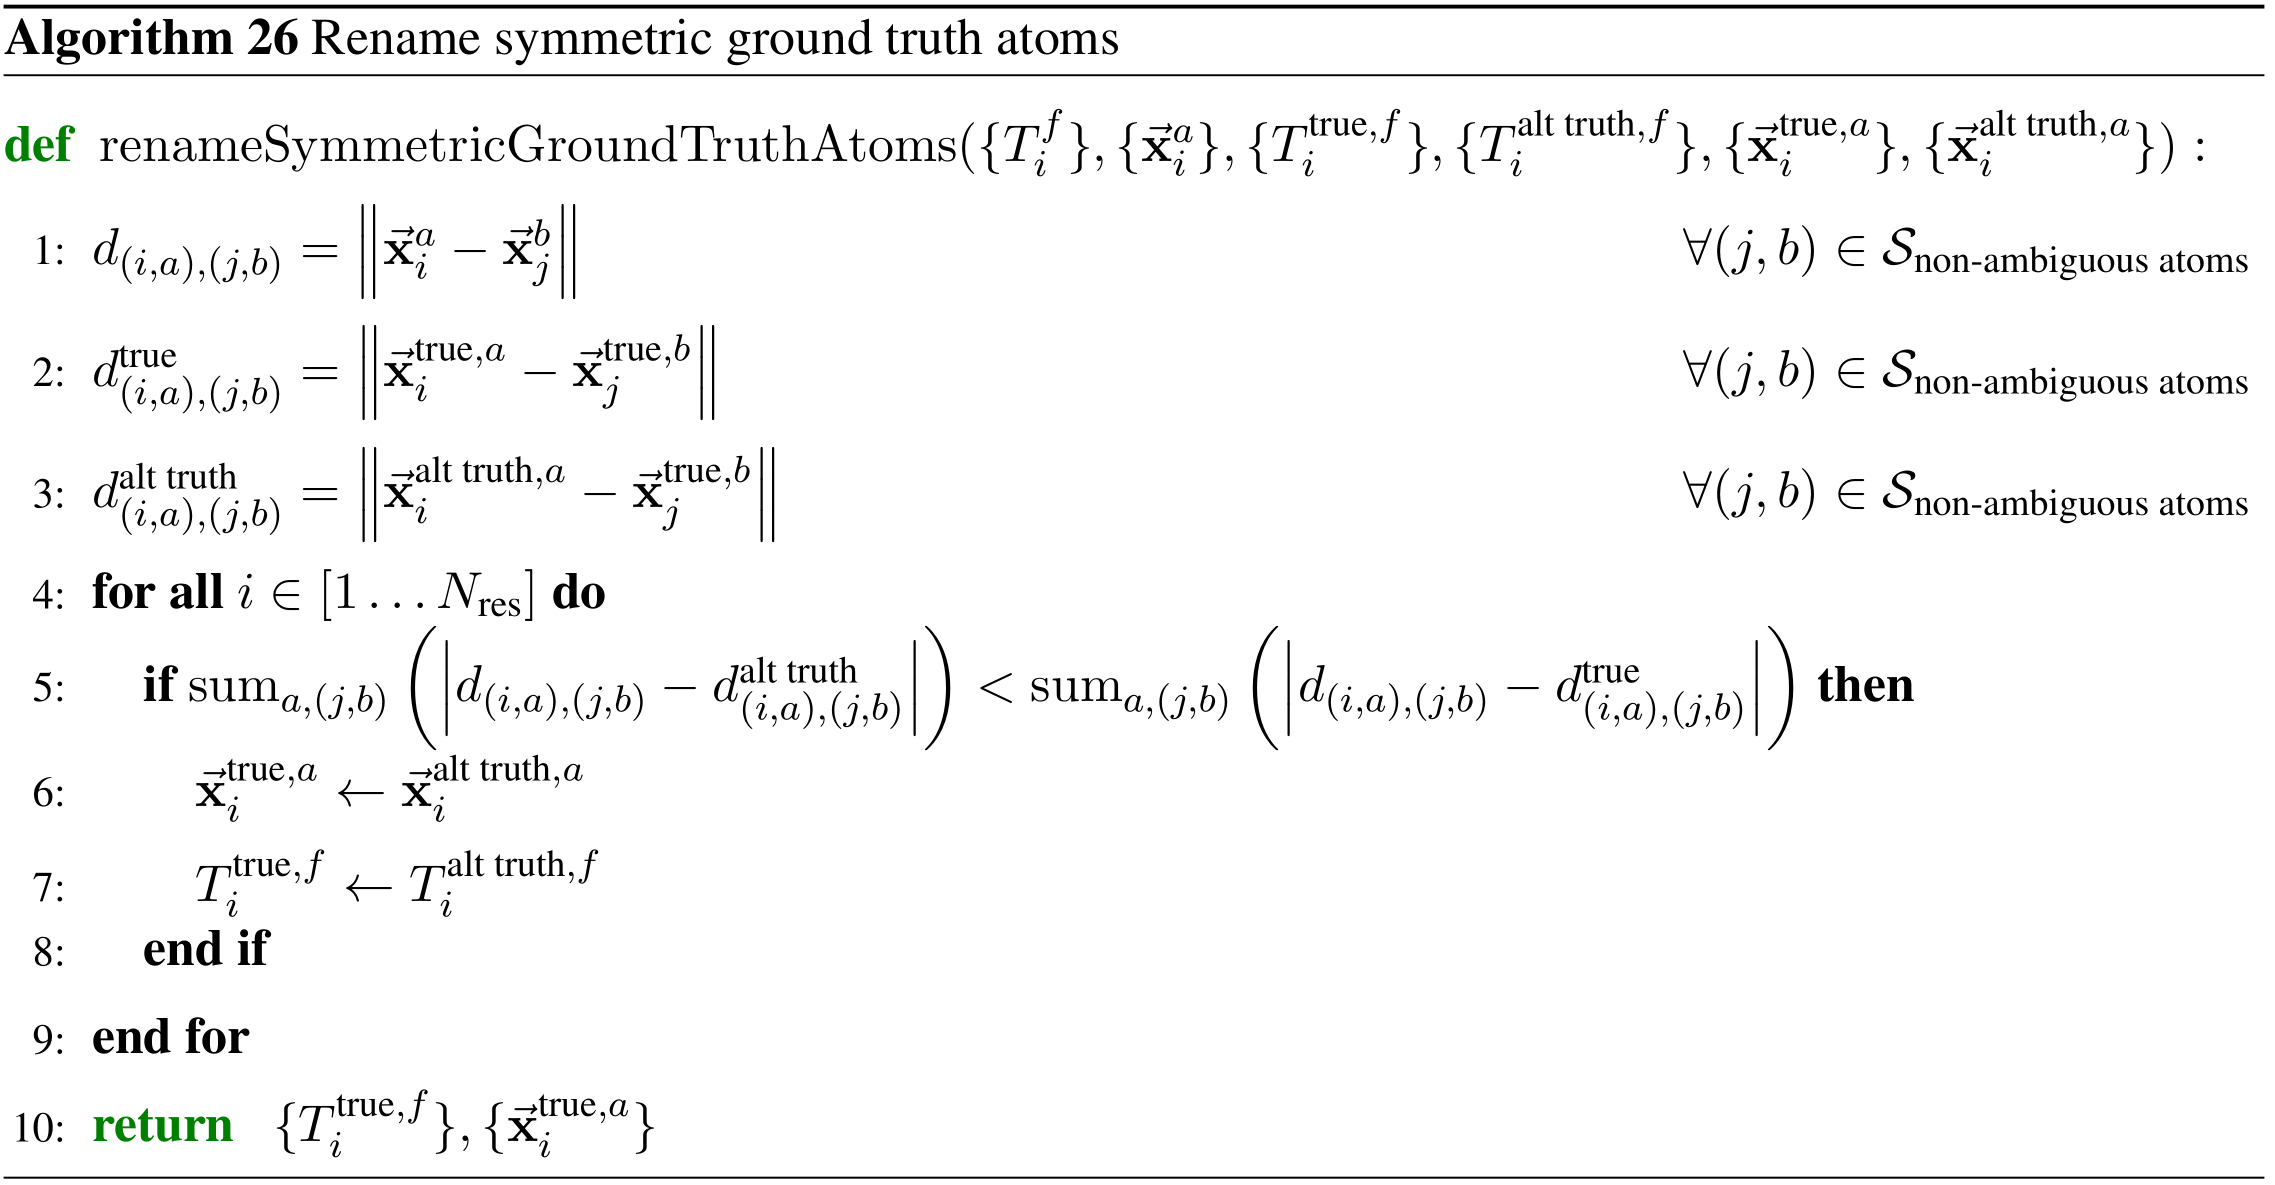
\includegraphics[width=.9\linewidth]{./imgs/rename-truth-atoms-algo26.png}
\end{center}
\end{frame}
\begin{frame}[label={sec:org6adb546}]{Algorithm 27 Side chain and backbone torsion angle loss \cite{jumperHighlyAccurateProtein2021}}
\begin{center}
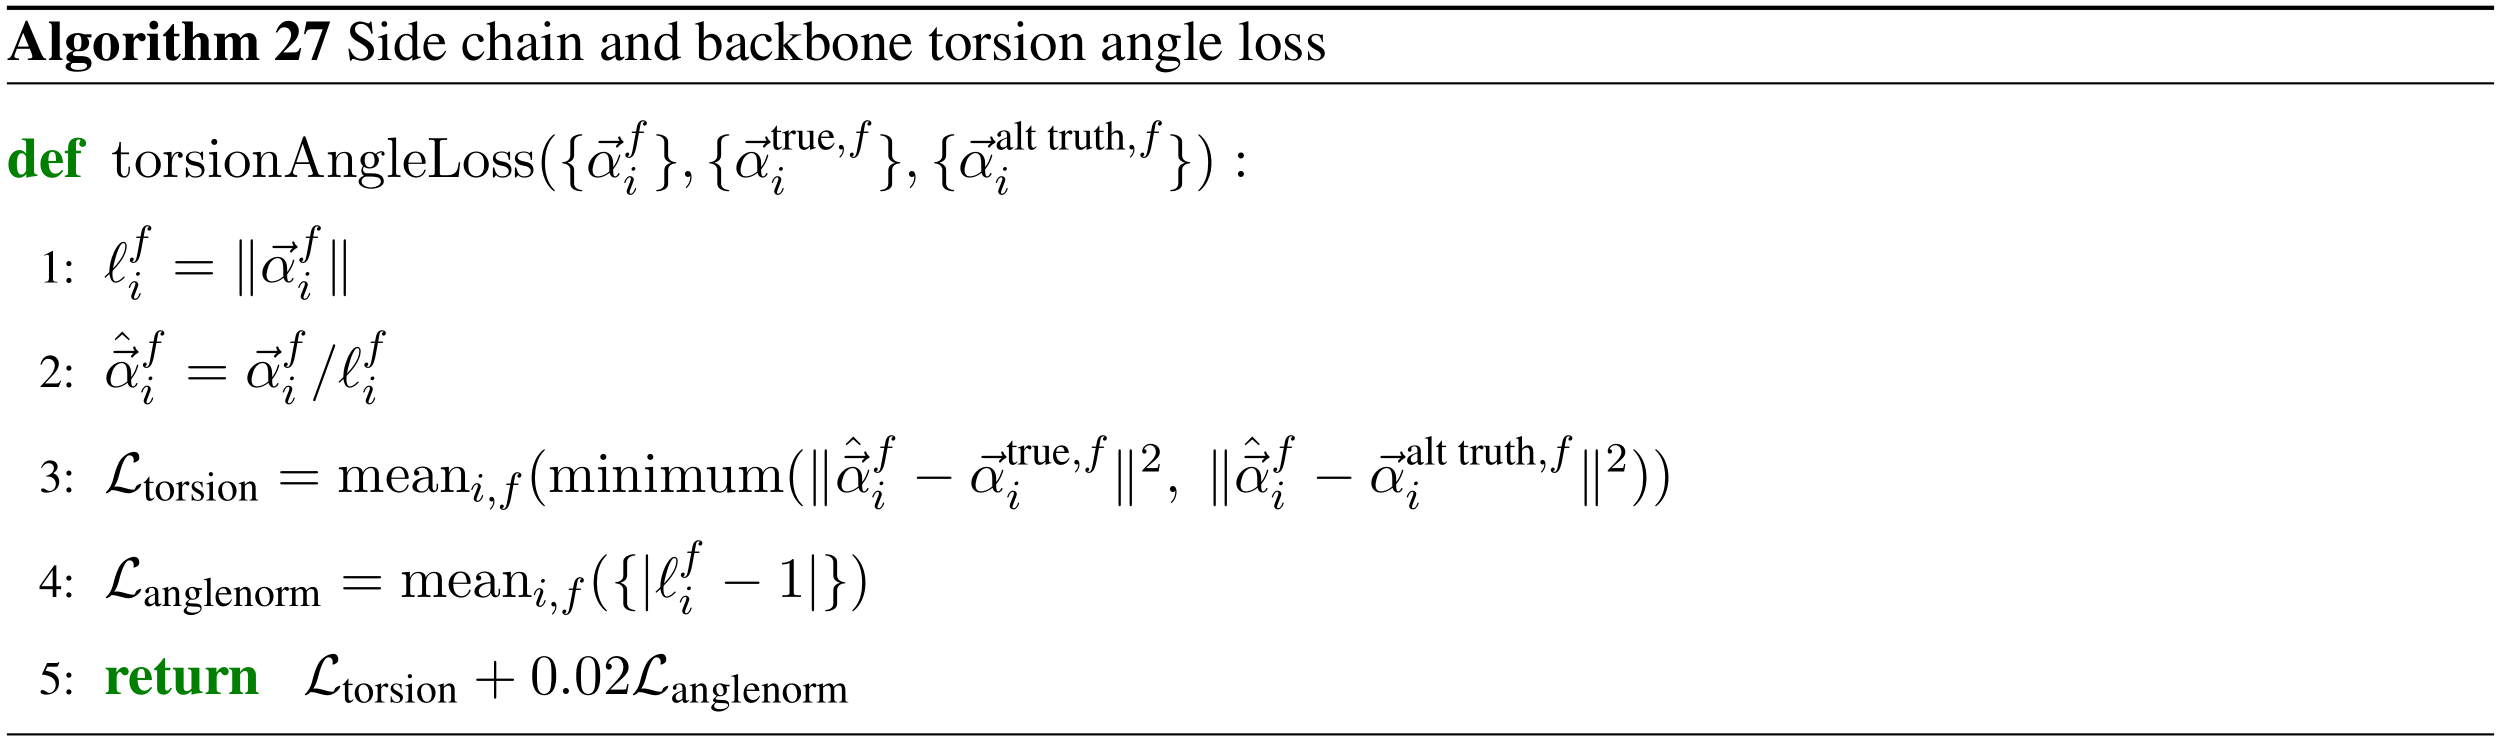
\includegraphics[width=.9\linewidth]{./imgs/sidechain-backbonetorsion-loss-algo27.png}
\end{center}
\end{frame}
\begin{frame}[label={sec:org30f2912}]{Algorithm 25 Make a transformation that rotates around the x-axis \cite{jumperHighlyAccurateProtein2021}}
\begin{center}
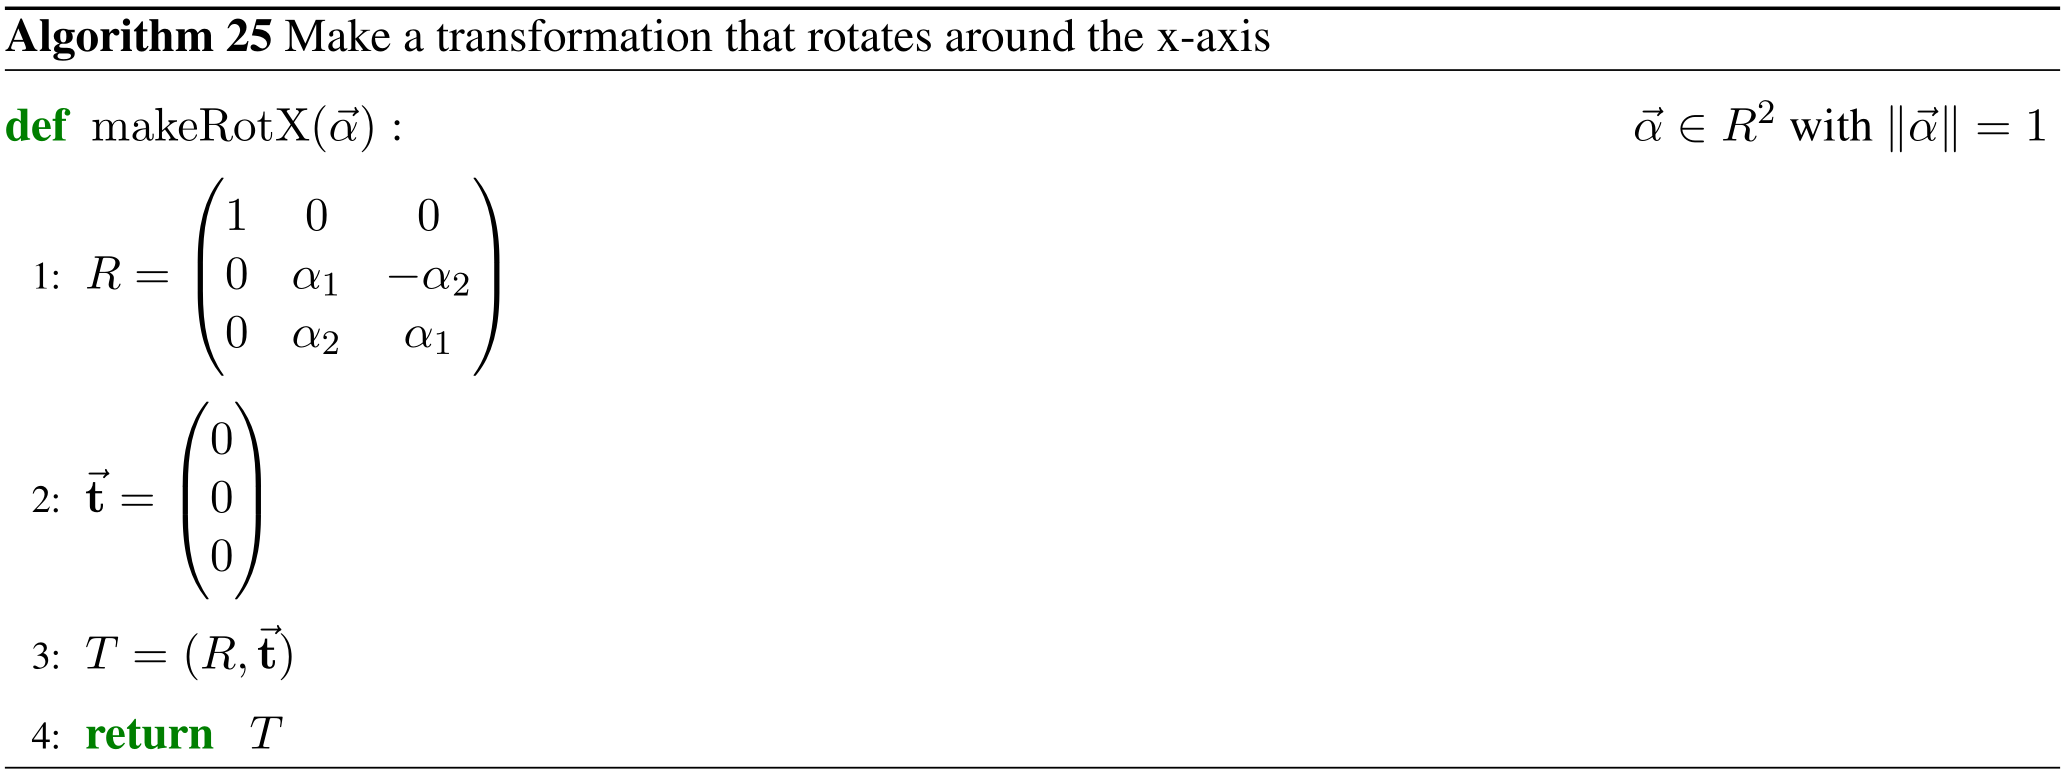
\includegraphics[width=.9\linewidth]{./imgs/xaxis-transform-algo.png}
\end{center}
\end{frame}
\section*{Biblio}
\label{sec:org2e8e00d}
\begin{frame}[fragile,allowframebreaks,label=]{Bibliography}
\printbibliography
\end{frame}
\end{document}